\documentclass [oneside,10pt,a4paper,ngerman,BCOR10mm,headsepline,parindent,final]{scrartcl}

    \usepackage[breakable]{tcolorbox}
    \usepackage{parskip} % Stop auto-indenting (to mimic markdown behaviour)
    

    % Basic figure setup, for now with no caption control since it's done
    % automatically by Pandoc (which extracts ![](path) syntax from Markdown).
    \usepackage{graphicx}
    % Maintain compatibility with old templates. Remove in nbconvert 6.0
    % \let\Oldincludegraphics\includegraphics
    % Ensure that by default, figures have no caption (until we provide a
    % proper Figure object with a Caption API and a way to capture that
    % in the conversion process - todo).
    % \usepackage{caption}
    % \DeclareCaptionFormat{nocaption}{}
    % \captionsetup{format=nocaption,aboveskip=0pt,belowskip=0pt}

    \usepackage{float}
    \floatplacement{figure}{H} % forces figures to be placed at the correct location
    \usepackage{xcolor} % Allow colors to be defined
    \usepackage{enumerate} % Needed for markdown enumerations to work
    \usepackage{geometry} % Used to adjust the document margins
    \usepackage{amsmath} % Equations
    \usepackage{amssymb} % Equations
    \usepackage{textcomp} % defines textquotesingle
    % Hack from http://tex.stackexchange.com/a/47451/13684:
    \AtBeginDocument{%
        \def\PYZsq{\textquotesingle}% Upright quotes in Pygmentized code
    }
    \usepackage{upquote} % Upright quotes for verbatim code
    \usepackage{eurosym} % defines \euro

    \usepackage{iftex}
    \ifPDFTeX
        \usepackage[T1]{fontenc}
        \usepackage[utf8]{inputenc}
    \else
        \usepackage{fontspec}
        \usepackage{unicode-math}
    \fi

    \usepackage{fancyvrb} % verbatim replacement that allows latex
    \usepackage{grffile} % extends the file name processing of package graphics 
                         % to support a larger range
    \makeatletter % fix for old versions of grffile with XeLaTeX
    \@ifpackagelater{grffile}{2019/11/01}
    {
      % Do nothing on new versions
    }
    {
      \def\Gread@@xetex#1{%
        \IfFileExists{"\Gin@base".bb}%
        {\Gread@eps{\Gin@base.bb}}%
        {\Gread@@xetex@aux#1}%
      }
    }
    \makeatother
    \usepackage[Export]{adjustbox} % Used to constrain images to a maximum size
    \adjustboxset{max size={0.9\linewidth}{0.9\paperheight}}

    % The hyperref package gives us a pdf with properly built
    % internal navigation ('pdf bookmarks' for the table of contents,
    % internal cross-reference links, web links for URLs, etc.)
    \usepackage{hyperref}
    % The default LaTeX title has an obnoxious amount of whitespace. By default,
    % titling removes some of it. It also provides customization options.
    \usepackage{titling}
    \usepackage{longtable} % longtable support required by pandoc >1.10
    \usepackage{booktabs}  % table support for pandoc > 1.12.2
    \usepackage{array}     % table support for pandoc >= 2.11.3
    \usepackage{calc}      % table minipage width calculation for pandoc >= 2.11.1
    \usepackage[inline]{enumitem} % IRkernel/repr support (it uses the enumerate* environment)
    \usepackage[normalem]{ulem} % ulem is needed to support strikethroughs (\sout)
                                % normalem makes italics be italics, not underlines
    \usepackage{mathrsfs}
    
    % Using fancy headers and footers
    \usepackage{fancyhdr}
    
    % Used for entering author names and their affiliations
    \usepackage[affil-it]{authblk}
    
    % Use bibliography% and configure it
    \usepackage[babel,german=quotes]{csquotes}
    \usepackage[backend=biber,style=authoryear,backref=true]{biblatex}
    \bibliography{literature/notebook.bib}
    \usepackage{url}                    %Output of nicely formatted Internet addresses
    \setcounter{biburllcpenalty}{7000}  %Setting for counter to wrap URLs in literature references
    \setcounter{biburlucpenalty}{8000}  %ditto



    
    % Colors for the hyperref package
    \definecolor{urlcolor}{rgb}{0,.145,.698}
    \definecolor{linkcolor}{rgb}{.71,0.21,0.01}
    \definecolor{citecolor}{rgb}{.12,.54,.11}

    % ANSI colors
    \definecolor{ansi-black}{HTML}{3E424D}
    \definecolor{ansi-black-intense}{HTML}{282C36}
    \definecolor{ansi-red}{HTML}{E75C58}
    \definecolor{ansi-red-intense}{HTML}{B22B31}
    \definecolor{ansi-green}{HTML}{00A250}
    \definecolor{ansi-green-intense}{HTML}{007427}
    \definecolor{ansi-yellow}{HTML}{DDB62B}
    \definecolor{ansi-yellow-intense}{HTML}{B27D12}
    \definecolor{ansi-blue}{HTML}{208FFB}
    \definecolor{ansi-blue-intense}{HTML}{0065CA}
    \definecolor{ansi-magenta}{HTML}{D160C4}
    \definecolor{ansi-magenta-intense}{HTML}{A03196}
    \definecolor{ansi-cyan}{HTML}{60C6C8}
    \definecolor{ansi-cyan-intense}{HTML}{258F8F}
    \definecolor{ansi-white}{HTML}{C5C1B4}
    \definecolor{ansi-white-intense}{HTML}{A1A6B2}
    \definecolor{ansi-default-inverse-fg}{HTML}{FFFFFF}
    \definecolor{ansi-default-inverse-bg}{HTML}{000000}

    % common color for the border for error outputs.
    \definecolor{outerrorbackground}{HTML}{FFDFDF}

    % commands and environments needed by pandoc snippets
    % extracted from the output of `pandoc -s`
    \providecommand{\tightlist}{%
      \setlength{\itemsep}{0pt}\setlength{\parskip}{0pt}}
    \DefineVerbatimEnvironment{Highlighting}{Verbatim}{commandchars=\\\{\}}
    % Add ',fontsize=\small' for more characters per line
    \newenvironment{Shaded}{}{}
    \newcommand{\KeywordTok}[1]{\textcolor[rgb]{0.00,0.44,0.13}{\textbf{{#1}}}}
    \newcommand{\DataTypeTok}[1]{\textcolor[rgb]{0.56,0.13,0.00}{{#1}}}
    \newcommand{\DecValTok}[1]{\textcolor[rgb]{0.25,0.63,0.44}{{#1}}}
    \newcommand{\BaseNTok}[1]{\textcolor[rgb]{0.25,0.63,0.44}{{#1}}}
    \newcommand{\FloatTok}[1]{\textcolor[rgb]{0.25,0.63,0.44}{{#1}}}
    \newcommand{\CharTok}[1]{\textcolor[rgb]{0.25,0.44,0.63}{{#1}}}
    \newcommand{\StringTok}[1]{\textcolor[rgb]{0.25,0.44,0.63}{{#1}}}
    \newcommand{\CommentTok}[1]{\textcolor[rgb]{0.38,0.63,0.69}{\textit{{#1}}}}
    \newcommand{\OtherTok}[1]{\textcolor[rgb]{0.00,0.44,0.13}{{#1}}}
    \newcommand{\AlertTok}[1]{\textcolor[rgb]{1.00,0.00,0.00}{\textbf{{#1}}}}
    \newcommand{\FunctionTok}[1]{\textcolor[rgb]{0.02,0.16,0.49}{{#1}}}
    \newcommand{\RegionMarkerTok}[1]{{#1}}
    \newcommand{\ErrorTok}[1]{\textcolor[rgb]{1.00,0.00,0.00}{\textbf{{#1}}}}
    \newcommand{\NormalTok}[1]{{#1}}
    
    % Additional commands for more recent versions of Pandoc
    \newcommand{\ConstantTok}[1]{\textcolor[rgb]{0.53,0.00,0.00}{{#1}}}
    \newcommand{\SpecialCharTok}[1]{\textcolor[rgb]{0.25,0.44,0.63}{{#1}}}
    \newcommand{\VerbatimStringTok}[1]{\textcolor[rgb]{0.25,0.44,0.63}{{#1}}}
    \newcommand{\SpecialStringTok}[1]{\textcolor[rgb]{0.73,0.40,0.53}{{#1}}}
    \newcommand{\ImportTok}[1]{{#1}}
    \newcommand{\DocumentationTok}[1]{\textcolor[rgb]{0.73,0.13,0.13}{\textit{{#1}}}}
    \newcommand{\AnnotationTok}[1]{\textcolor[rgb]{0.38,0.63,0.69}{\textbf{\textit{{#1}}}}}
    \newcommand{\CommentVarTok}[1]{\textcolor[rgb]{0.38,0.63,0.69}{\textbf{\textit{{#1}}}}}
    \newcommand{\VariableTok}[1]{\textcolor[rgb]{0.10,0.09,0.49}{{#1}}}
    \newcommand{\ControlFlowTok}[1]{\textcolor[rgb]{0.00,0.44,0.13}{\textbf{{#1}}}}
    \newcommand{\OperatorTok}[1]{\textcolor[rgb]{0.40,0.40,0.40}{{#1}}}
    \newcommand{\BuiltInTok}[1]{{#1}}
    \newcommand{\ExtensionTok}[1]{{#1}}
    \newcommand{\PreprocessorTok}[1]{\textcolor[rgb]{0.74,0.48,0.00}{{#1}}}
    \newcommand{\AttributeTok}[1]{\textcolor[rgb]{0.49,0.56,0.16}{{#1}}}
    \newcommand{\InformationTok}[1]{\textcolor[rgb]{0.38,0.63,0.69}{\textbf{\textit{{#1}}}}}
    \newcommand{\WarningTok}[1]{\textcolor[rgb]{0.38,0.63,0.69}{\textbf{\textit{{#1}}}}}
    
    
    % Define a nice break command that doesn't care if a line doesn't already
    % exist.
    \def\br{\hspace*{\fill} \\* }
    % Math Jax compatibility definitions
    \def\gt{>}
    \def\lt{<}
    \let\Oldtex\TeX
    \let\Oldlatex\LaTeX
    \renewcommand{\TeX}{\textrm{\Oldtex}}
    \renewcommand{\LaTeX}{\textrm{\Oldlatex}}
    % Document parameters
    % Document title
    \title{\textbf{\textsf{Application of the processed survey data in the analytical hierarchy process (AHP)}}}\author[1]{Bj\"orn Kasper (\href{mailto:kasper.bjoern@bgetem.de}{kasper.bjoern@bgetem.de})}
\affil[1]{Berufsgenossenschaft Energie Textil Elektro Medienerzeugnisse}\author[2]{Henriette John (\href{mailto:h.john@ioer.de}{h.john@ioer.de})}
\affil[2]{Leibniz Institute of Ecological Urban and Regional Development}\date{\today; version 0.1 (pre-release)}


    
    
    
    
    
% Pygments definitions
\makeatletter
\def\PY@reset{\let\PY@it=\relax \let\PY@bf=\relax%
    \let\PY@ul=\relax \let\PY@tc=\relax%
    \let\PY@bc=\relax \let\PY@ff=\relax}
\def\PY@tok#1{\csname PY@tok@#1\endcsname}
\def\PY@toks#1+{\ifx\relax#1\empty\else%
    \PY@tok{#1}\expandafter\PY@toks\fi}
\def\PY@do#1{\PY@bc{\PY@tc{\PY@ul{%
    \PY@it{\PY@bf{\PY@ff{#1}}}}}}}
\def\PY#1#2{\PY@reset\PY@toks#1+\relax+\PY@do{#2}}

\@namedef{PY@tok@w}{\def\PY@tc##1{\textcolor[rgb]{0.73,0.73,0.73}{##1}}}
\@namedef{PY@tok@c}{\let\PY@it=\textit\def\PY@tc##1{\textcolor[rgb]{0.24,0.48,0.48}{##1}}}
\@namedef{PY@tok@cp}{\def\PY@tc##1{\textcolor[rgb]{0.61,0.40,0.00}{##1}}}
\@namedef{PY@tok@k}{\let\PY@bf=\textbf\def\PY@tc##1{\textcolor[rgb]{0.00,0.50,0.00}{##1}}}
\@namedef{PY@tok@kp}{\def\PY@tc##1{\textcolor[rgb]{0.00,0.50,0.00}{##1}}}
\@namedef{PY@tok@kt}{\def\PY@tc##1{\textcolor[rgb]{0.69,0.00,0.25}{##1}}}
\@namedef{PY@tok@o}{\def\PY@tc##1{\textcolor[rgb]{0.40,0.40,0.40}{##1}}}
\@namedef{PY@tok@ow}{\let\PY@bf=\textbf\def\PY@tc##1{\textcolor[rgb]{0.67,0.13,1.00}{##1}}}
\@namedef{PY@tok@nb}{\def\PY@tc##1{\textcolor[rgb]{0.00,0.50,0.00}{##1}}}
\@namedef{PY@tok@nf}{\def\PY@tc##1{\textcolor[rgb]{0.00,0.00,1.00}{##1}}}
\@namedef{PY@tok@nc}{\let\PY@bf=\textbf\def\PY@tc##1{\textcolor[rgb]{0.00,0.00,1.00}{##1}}}
\@namedef{PY@tok@nn}{\let\PY@bf=\textbf\def\PY@tc##1{\textcolor[rgb]{0.00,0.00,1.00}{##1}}}
\@namedef{PY@tok@ne}{\let\PY@bf=\textbf\def\PY@tc##1{\textcolor[rgb]{0.80,0.25,0.22}{##1}}}
\@namedef{PY@tok@nv}{\def\PY@tc##1{\textcolor[rgb]{0.10,0.09,0.49}{##1}}}
\@namedef{PY@tok@no}{\def\PY@tc##1{\textcolor[rgb]{0.53,0.00,0.00}{##1}}}
\@namedef{PY@tok@nl}{\def\PY@tc##1{\textcolor[rgb]{0.46,0.46,0.00}{##1}}}
\@namedef{PY@tok@ni}{\let\PY@bf=\textbf\def\PY@tc##1{\textcolor[rgb]{0.44,0.44,0.44}{##1}}}
\@namedef{PY@tok@na}{\def\PY@tc##1{\textcolor[rgb]{0.41,0.47,0.13}{##1}}}
\@namedef{PY@tok@nt}{\let\PY@bf=\textbf\def\PY@tc##1{\textcolor[rgb]{0.00,0.50,0.00}{##1}}}
\@namedef{PY@tok@nd}{\def\PY@tc##1{\textcolor[rgb]{0.67,0.13,1.00}{##1}}}
\@namedef{PY@tok@s}{\def\PY@tc##1{\textcolor[rgb]{0.73,0.13,0.13}{##1}}}
\@namedef{PY@tok@sd}{\let\PY@it=\textit\def\PY@tc##1{\textcolor[rgb]{0.73,0.13,0.13}{##1}}}
\@namedef{PY@tok@si}{\let\PY@bf=\textbf\def\PY@tc##1{\textcolor[rgb]{0.64,0.35,0.47}{##1}}}
\@namedef{PY@tok@se}{\let\PY@bf=\textbf\def\PY@tc##1{\textcolor[rgb]{0.67,0.36,0.12}{##1}}}
\@namedef{PY@tok@sr}{\def\PY@tc##1{\textcolor[rgb]{0.64,0.35,0.47}{##1}}}
\@namedef{PY@tok@ss}{\def\PY@tc##1{\textcolor[rgb]{0.10,0.09,0.49}{##1}}}
\@namedef{PY@tok@sx}{\def\PY@tc##1{\textcolor[rgb]{0.00,0.50,0.00}{##1}}}
\@namedef{PY@tok@m}{\def\PY@tc##1{\textcolor[rgb]{0.40,0.40,0.40}{##1}}}
\@namedef{PY@tok@gh}{\let\PY@bf=\textbf\def\PY@tc##1{\textcolor[rgb]{0.00,0.00,0.50}{##1}}}
\@namedef{PY@tok@gu}{\let\PY@bf=\textbf\def\PY@tc##1{\textcolor[rgb]{0.50,0.00,0.50}{##1}}}
\@namedef{PY@tok@gd}{\def\PY@tc##1{\textcolor[rgb]{0.63,0.00,0.00}{##1}}}
\@namedef{PY@tok@gi}{\def\PY@tc##1{\textcolor[rgb]{0.00,0.52,0.00}{##1}}}
\@namedef{PY@tok@gr}{\def\PY@tc##1{\textcolor[rgb]{0.89,0.00,0.00}{##1}}}
\@namedef{PY@tok@ge}{\let\PY@it=\textit}
\@namedef{PY@tok@gs}{\let\PY@bf=\textbf}
\@namedef{PY@tok@gp}{\let\PY@bf=\textbf\def\PY@tc##1{\textcolor[rgb]{0.00,0.00,0.50}{##1}}}
\@namedef{PY@tok@go}{\def\PY@tc##1{\textcolor[rgb]{0.44,0.44,0.44}{##1}}}
\@namedef{PY@tok@gt}{\def\PY@tc##1{\textcolor[rgb]{0.00,0.27,0.87}{##1}}}
\@namedef{PY@tok@err}{\def\PY@bc##1{{\setlength{\fboxsep}{\string -\fboxrule}\fcolorbox[rgb]{1.00,0.00,0.00}{1,1,1}{\strut ##1}}}}
\@namedef{PY@tok@kc}{\let\PY@bf=\textbf\def\PY@tc##1{\textcolor[rgb]{0.00,0.50,0.00}{##1}}}
\@namedef{PY@tok@kd}{\let\PY@bf=\textbf\def\PY@tc##1{\textcolor[rgb]{0.00,0.50,0.00}{##1}}}
\@namedef{PY@tok@kn}{\let\PY@bf=\textbf\def\PY@tc##1{\textcolor[rgb]{0.00,0.50,0.00}{##1}}}
\@namedef{PY@tok@kr}{\let\PY@bf=\textbf\def\PY@tc##1{\textcolor[rgb]{0.00,0.50,0.00}{##1}}}
\@namedef{PY@tok@bp}{\def\PY@tc##1{\textcolor[rgb]{0.00,0.50,0.00}{##1}}}
\@namedef{PY@tok@fm}{\def\PY@tc##1{\textcolor[rgb]{0.00,0.00,1.00}{##1}}}
\@namedef{PY@tok@vc}{\def\PY@tc##1{\textcolor[rgb]{0.10,0.09,0.49}{##1}}}
\@namedef{PY@tok@vg}{\def\PY@tc##1{\textcolor[rgb]{0.10,0.09,0.49}{##1}}}
\@namedef{PY@tok@vi}{\def\PY@tc##1{\textcolor[rgb]{0.10,0.09,0.49}{##1}}}
\@namedef{PY@tok@vm}{\def\PY@tc##1{\textcolor[rgb]{0.10,0.09,0.49}{##1}}}
\@namedef{PY@tok@sa}{\def\PY@tc##1{\textcolor[rgb]{0.73,0.13,0.13}{##1}}}
\@namedef{PY@tok@sb}{\def\PY@tc##1{\textcolor[rgb]{0.73,0.13,0.13}{##1}}}
\@namedef{PY@tok@sc}{\def\PY@tc##1{\textcolor[rgb]{0.73,0.13,0.13}{##1}}}
\@namedef{PY@tok@dl}{\def\PY@tc##1{\textcolor[rgb]{0.73,0.13,0.13}{##1}}}
\@namedef{PY@tok@s2}{\def\PY@tc##1{\textcolor[rgb]{0.73,0.13,0.13}{##1}}}
\@namedef{PY@tok@sh}{\def\PY@tc##1{\textcolor[rgb]{0.73,0.13,0.13}{##1}}}
\@namedef{PY@tok@s1}{\def\PY@tc##1{\textcolor[rgb]{0.73,0.13,0.13}{##1}}}
\@namedef{PY@tok@mb}{\def\PY@tc##1{\textcolor[rgb]{0.40,0.40,0.40}{##1}}}
\@namedef{PY@tok@mf}{\def\PY@tc##1{\textcolor[rgb]{0.40,0.40,0.40}{##1}}}
\@namedef{PY@tok@mh}{\def\PY@tc##1{\textcolor[rgb]{0.40,0.40,0.40}{##1}}}
\@namedef{PY@tok@mi}{\def\PY@tc##1{\textcolor[rgb]{0.40,0.40,0.40}{##1}}}
\@namedef{PY@tok@il}{\def\PY@tc##1{\textcolor[rgb]{0.40,0.40,0.40}{##1}}}
\@namedef{PY@tok@mo}{\def\PY@tc##1{\textcolor[rgb]{0.40,0.40,0.40}{##1}}}
\@namedef{PY@tok@ch}{\let\PY@it=\textit\def\PY@tc##1{\textcolor[rgb]{0.24,0.48,0.48}{##1}}}
\@namedef{PY@tok@cm}{\let\PY@it=\textit\def\PY@tc##1{\textcolor[rgb]{0.24,0.48,0.48}{##1}}}
\@namedef{PY@tok@cpf}{\let\PY@it=\textit\def\PY@tc##1{\textcolor[rgb]{0.24,0.48,0.48}{##1}}}
\@namedef{PY@tok@c1}{\let\PY@it=\textit\def\PY@tc##1{\textcolor[rgb]{0.24,0.48,0.48}{##1}}}
\@namedef{PY@tok@cs}{\let\PY@it=\textit\def\PY@tc##1{\textcolor[rgb]{0.24,0.48,0.48}{##1}}}

\def\PYZbs{\char`\\}
\def\PYZus{\char`\_}
\def\PYZob{\char`\{}
\def\PYZcb{\char`\}}
\def\PYZca{\char`\^}
\def\PYZam{\char`\&}
\def\PYZlt{\char`\<}
\def\PYZgt{\char`\>}
\def\PYZsh{\char`\#}
\def\PYZpc{\char`\%}
\def\PYZdl{\char`\$}
\def\PYZhy{\char`\-}
\def\PYZsq{\char`\'}
\def\PYZdq{\char`\"}
\def\PYZti{\char`\~}
% for compatibility with earlier versions
\def\PYZat{@}
\def\PYZlb{[}
\def\PYZrb{]}
\makeatother


    % For linebreaks inside Verbatim environment from package fancyvrb. 
    \makeatletter
        \newbox\Wrappedcontinuationbox 
        \newbox\Wrappedvisiblespacebox 
        \newcommand*\Wrappedvisiblespace {\textcolor{red}{\textvisiblespace}} 
        \newcommand*\Wrappedcontinuationsymbol {\textcolor{red}{\llap{\tiny$\m@th\hookrightarrow$}}} 
        \newcommand*\Wrappedcontinuationindent {3ex } 
        \newcommand*\Wrappedafterbreak {\kern\Wrappedcontinuationindent\copy\Wrappedcontinuationbox} 
        % Take advantage of the already applied Pygments mark-up to insert 
        % potential linebreaks for TeX processing. 
        %        {, <, #, %, $, ' and ": go to next line. 
        %        _, }, ^, &, >, - and ~: stay at end of broken line. 
        % Use of \textquotesingle for straight quote. 
        \newcommand*\Wrappedbreaksatspecials {% 
            \def\PYGZus{\discretionary{\char`\_}{\Wrappedafterbreak}{\char`\_}}% 
            \def\PYGZob{\discretionary{}{\Wrappedafterbreak\char`\{}{\char`\{}}% 
            \def\PYGZcb{\discretionary{\char`\}}{\Wrappedafterbreak}{\char`\}}}% 
            \def\PYGZca{\discretionary{\char`\^}{\Wrappedafterbreak}{\char`\^}}% 
            \def\PYGZam{\discretionary{\char`\&}{\Wrappedafterbreak}{\char`\&}}% 
            \def\PYGZlt{\discretionary{}{\Wrappedafterbreak\char`\<}{\char`\<}}% 
            \def\PYGZgt{\discretionary{\char`\>}{\Wrappedafterbreak}{\char`\>}}% 
            \def\PYGZsh{\discretionary{}{\Wrappedafterbreak\char`\#}{\char`\#}}% 
            \def\PYGZpc{\discretionary{}{\Wrappedafterbreak\char`\%}{\char`\%}}% 
            \def\PYGZdl{\discretionary{}{\Wrappedafterbreak\char`\$}{\char`\$}}% 
            \def\PYGZhy{\discretionary{\char`\-}{\Wrappedafterbreak}{\char`\-}}% 
            \def\PYGZsq{\discretionary{}{\Wrappedafterbreak\textquotesingle}{\textquotesingle}}% 
            \def\PYGZdq{\discretionary{}{\Wrappedafterbreak\char`\"}{\char`\"}}% 
            \def\PYGZti{\discretionary{\char`\~}{\Wrappedafterbreak}{\char`\~}}% 
        } 
        % Some characters . , ; ? ! / are not pygmentized. 
        % This macro makes them "active" and they will insert potential linebreaks 
        \newcommand*\Wrappedbreaksatpunct {% 
            \lccode`\~`\.\lowercase{\def~}{\discretionary{\hbox{\char`\.}}{\Wrappedafterbreak}{\hbox{\char`\.}}}% 
            \lccode`\~`\,\lowercase{\def~}{\discretionary{\hbox{\char`\,}}{\Wrappedafterbreak}{\hbox{\char`\,}}}% 
            \lccode`\~`\;\lowercase{\def~}{\discretionary{\hbox{\char`\;}}{\Wrappedafterbreak}{\hbox{\char`\;}}}% 
            \lccode`\~`\:\lowercase{\def~}{\discretionary{\hbox{\char`\:}}{\Wrappedafterbreak}{\hbox{\char`\:}}}% 
            \lccode`\~`\?\lowercase{\def~}{\discretionary{\hbox{\char`\?}}{\Wrappedafterbreak}{\hbox{\char`\?}}}% 
            \lccode`\~`\!\lowercase{\def~}{\discretionary{\hbox{\char`\!}}{\Wrappedafterbreak}{\hbox{\char`\!}}}% 
            \lccode`\~`\/\lowercase{\def~}{\discretionary{\hbox{\char`\/}}{\Wrappedafterbreak}{\hbox{\char`\/}}}% 
            \catcode`\.\active
            \catcode`\,\active 
            \catcode`\;\active
            \catcode`\:\active
            \catcode`\?\active
            \catcode`\!\active
            \catcode`\/\active 
            \lccode`\~`\~ 	
        }
    \makeatother

    \let\OriginalVerbatim=\Verbatim
    \makeatletter
    \renewcommand{\Verbatim}[1][1]{%
        %\parskip\z@skip
        \sbox\Wrappedcontinuationbox {\Wrappedcontinuationsymbol}%
        \sbox\Wrappedvisiblespacebox {\FV@SetupFont\Wrappedvisiblespace}%
        \def\FancyVerbFormatLine ##1{\hsize\linewidth
            \vtop{\raggedright\hyphenpenalty\z@\exhyphenpenalty\z@
                \doublehyphendemerits\z@\finalhyphendemerits\z@
                \strut ##1\strut}%
        }%
        % If the linebreak is at a space, the latter will be displayed as visible
        % space at end of first line, and a continuation symbol starts next line.
        % Stretch/shrink are however usually zero for typewriter font.
        \def\FV@Space {%
            \nobreak\hskip\z@ plus\fontdimen3\font minus\fontdimen4\font
            \discretionary{\copy\Wrappedvisiblespacebox}{\Wrappedafterbreak}
            {\kern\fontdimen2\font}%
        }%
        
        % Allow breaks at special characters using \PYG... macros.
        \Wrappedbreaksatspecials
        % Breaks at punctuation characters . , ; ? ! and / need catcode=\active 	
        \OriginalVerbatim[#1,codes*=\Wrappedbreaksatpunct]%
    }
    \makeatother

    % Exact colors from NB
    \definecolor{incolor}{HTML}{303F9F}
    \definecolor{outcolor}{HTML}{D84315}
    \definecolor{cellborder}{HTML}{CFCFCF}
    \definecolor{cellbackground}{HTML}{F7F7F7}
    
    % prompt
    \makeatletter
    \newcommand{\boxspacing}{\kern\kvtcb@left@rule\kern\kvtcb@boxsep}
    \makeatother
    \newcommand{\prompt}[4]{
        {\ttfamily\llap{{\color{#2}[#3]:\hspace{3pt}#4}}\vspace{-\baselineskip}}
    }
    

    
    % Prevent overflowing lines due to hard-to-break entities
    \sloppy

    % Setup hyperref package
    \hypersetup{
      breaklinks=true,  % so long urls are correctly broken across lines
      bookmarksnumbered=true,
      pdfauthor=Bj\"orn Kasper,
      pdftitle=Application of the processed survey data in the analytical hierarchy process (AHP),
      colorlinks=true,
      urlcolor=urlcolor,
      linkcolor=linkcolor,
      citecolor=citecolor,
      pdfpagemode={UseOutlines},
      pdfview = {XYZ},
      pdfstartview = {XYZ},
      pdfstartpage = {1},
      pdfborder={0 0 0}
      }
    % Slightly bigger margins than the latex defaults
    \geometry{verbose,tmargin=1in,bmargin=1in,lmargin=1in,rmargin=1in}



\begin{document}
    
    % Without changing the numbering style,
    % page numbers and column titles should be turned off.
    \pagestyle{empty}
    
    \maketitle\thispagestyle{empty}\begin{center}
        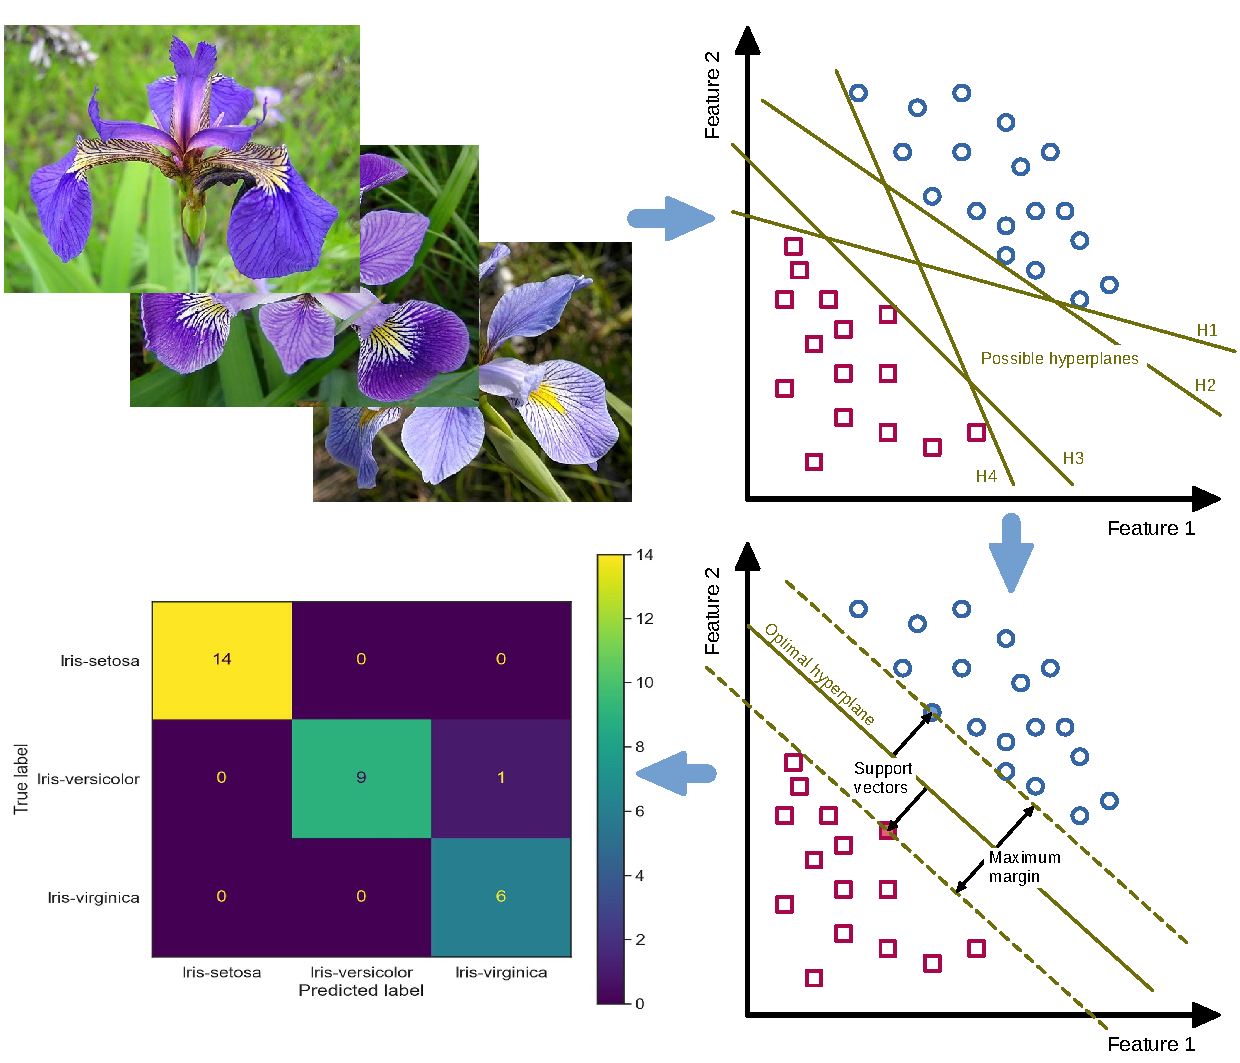
\includegraphics[width=0.90\textwidth]{images/Cover_image.pdf}
        \end{center}
        \vfill

    \begin{abstract}
    This is a placeholder for the abstract that needs to be added later.
    \end{abstract}
    \vfill

    \newpage

    % Activate own page style
    \pagestyle{fancy}
    % Delete all fields
    \fancyhf{}
    % \fancyhead[EL,OL]{$header$}
    % \fancyfoot[EL,OL]{$footer$}
    % Header leftside: chapter/section
    \fancyhead[ER,OR]{\leftmark}
    % Footer rightside: page number
    \fancyfoot[ER,OR]{Seite \thepage}

    \renewcommand{\sectionmark}[1]{
        \markboth{\thesection{} #1}{}
    }

    
    \tableofcontents
    
    


    
    \hypertarget{introduction}{%
\section{Introduction}\label{introduction}}

Why we use a
\href{https://en.wikipedia.org/wiki/Project_Jupyter}{Jupyter} notebook
to to publish the R program examples:

Jupyter is a new \textbf{open source} alternative to the proprietary
numerical software
\href{https://en.wikipedia.org/wiki/Wolfram_Mathematica}{Mathematica}
from \textbf{Wolfram Research} that is well on the way to become a
\textbf{standard for exchanging research results}
(\cite{Scientific_Paper_obsolete_2018};
\cite{Future_of_Research_Paper_2018}).

Originally Jupyter was intended as an IDE for the programming languages
\textbf{Julia} and \textbf{Python}. Besides that it is also possible to
install other interpreter kernels, such as the
\textbf{\href{https://irkernel.github.io/installation/}{IRkernel}} for
R. This can be interesting if the IDE \textbf{RStudio Desktop} is not
available on the target platform used. For example, it is very difficult
to install RStudio on the ARM-based embedded computer \textbf{Raspberry
Pi} due to many technical dependencies. In contrast, using the R kernel
in JupyterLab on the Raspberry Pi works very well and performant.

    \hypertarget{global-settings-and-dependencies}{%
\section{Global settings and
dependencies}\label{global-settings-and-dependencies}}

\hypertarget{install-missing-packages-if-not-present-yet}{%
\subsection{Install missing packages if not present
yet}\label{install-missing-packages-if-not-present-yet}}

\textbf{Attention:} For some R packages several dependencies have to be
installed first with
\texttt{apt\ install\ \textless{}package\ name\textgreater{}}.

Dependencies for package \texttt{ahpsurvey}:\\
- R package \texttt{randomNames} (it depends on R ≥ 4.0, refer to
\url{https://cran.r-project.org/web/packages/randomNames/index.html})

Drawback for \textbf{Raspbian buster}: the dependency
\texttt{randomNames} is not available for R v3.5.2 as it depends on R (≥
4.0). Upgrading R in Raspbian following the instruction on
\url{https://cran.rstudio.com/bin/linux/debian/\#debian-buster-stable}
does not work so far \ldots{}

    \begin{tcolorbox}[breakable, size=fbox, boxrule=1pt, pad at break*=1mm,colback=cellbackground, colframe=cellborder]
\prompt{In}{incolor}{132}{\boxspacing}
\begin{Verbatim}[commandchars=\\\{\}]
\PY{c+c1}{\PYZsh{} List of R packages that are used in this script}
\PY{n}{list.of.packages} \PY{o}{\PYZlt{}\PYZhy{}} \PY{n+nf}{c}\PY{p}{(}\PY{l+s}{\PYZdq{}}\PY{l+s}{data.table\PYZdq{}}\PY{p}{,} \PY{l+s}{\PYZdq{}}\PY{l+s}{ggplot2\PYZdq{}}\PY{p}{,} \PY{l+s}{\PYZdq{}}\PY{l+s}{tidyr\PYZdq{}}\PY{p}{,} \PY{l+s}{\PYZdq{}}\PY{l+s}{dplyr\PYZdq{}}\PY{p}{,} \PY{l+s}{\PYZdq{}}\PY{l+s}{magrittr\PYZdq{}}\PY{p}{,} \PY{l+s}{\PYZdq{}}\PY{l+s}{ahpsurvey\PYZdq{}}\PY{p}{,} \PY{l+s}{\PYZdq{}}\PY{l+s}{knitr\PYZdq{}}\PY{p}{,} \PY{l+s}{\PYZdq{}}\PY{l+s}{IRdisplay\PYZdq{}}\PY{p}{,} \PY{l+s}{\PYZdq{}}\PY{l+s}{forcats\PYZdq{}}\PY{p}{)}

\PY{c+c1}{\PYZsh{} Query the already installed packages and save the missing ones in a new list}
\PY{n}{missing.packages} \PY{o}{\PYZlt{}\PYZhy{}} \PY{n}{list.of.packages}\PY{p}{[}\PY{o}{!}\PY{p}{(}\PY{n}{list.of.packages} \PY{o}{\PYZpc{}in\PYZpc{}} \PY{n+nf}{installed.packages}\PY{p}{(}\PY{p}{)}\PY{p}{[}\PY{p}{,}\PY{l+s}{\PYZdq{}}\PY{l+s}{Package\PYZdq{}}\PY{p}{]}\PY{p}{)}\PY{p}{]}

\PY{c+c1}{\PYZsh{} Install missing packages}
\PY{n+nf}{if}\PY{p}{(}\PY{n+nf}{length}\PY{p}{(}\PY{n}{missing.packages}\PY{p}{)}\PY{p}{)} \PY{p}{\PYZob{}}
    \PY{n+nf}{install.packages}\PY{p}{(}\PY{n}{missing.packages}\PY{p}{)}
\PY{p}{\PYZcb{}} \PY{n}{else} \PY{p}{\PYZob{}}
    \PY{n+nf}{print}\PY{p}{(}\PY{l+s}{\PYZdq{}}\PY{l+s}{All required packages are installed.\PYZdq{}}\PY{p}{)}
\PY{p}{\PYZcb{}}
\end{Verbatim}
\end{tcolorbox}

    \begin{Verbatim}[commandchars=\\\{\}]
[1] "All required packages are installed."
    \end{Verbatim}

    \hypertarget{load-package-data.table}{%
\subsection{\texorpdfstring{Load package
\texttt{data.table}}{Load package data.table}}\label{load-package-data.table}}

The package \texttt{data.table} is used to read and manipulate tables
(\texttt{data.table} inherits from \texttt{data.frame}). Install and
load it:

    \begin{tcolorbox}[breakable, size=fbox, boxrule=1pt, pad at break*=1mm,colback=cellbackground, colframe=cellborder]
\prompt{In}{incolor}{2}{\boxspacing}
\begin{Verbatim}[commandchars=\\\{\}]
\PY{n+nf}{library}\PY{p}{(}\PY{n}{data.table}\PY{p}{)}
\end{Verbatim}
\end{tcolorbox}

    \hypertarget{load-package-ggplot2}{%
\subsection{\texorpdfstring{Load package
\texttt{ggplot2}}{Load package ggplot2}}\label{load-package-ggplot2}}

The package \texttt{ggplot2} is used to plot diagrams. Install and load
it:

    \begin{tcolorbox}[breakable, size=fbox, boxrule=1pt, pad at break*=1mm,colback=cellbackground, colframe=cellborder]
\prompt{In}{incolor}{3}{\boxspacing}
\begin{Verbatim}[commandchars=\\\{\}]
\PY{n+nf}{library}\PY{p}{(}\PY{n}{ggplot2}\PY{p}{)}
\end{Verbatim}
\end{tcolorbox}

    \hypertarget{load-packages-knitr-and-irdisplay}{%
\subsection{\texorpdfstring{Load packages \texttt{knitr} and
\texttt{IRdisplay}}{Load packages knitr and IRdisplay}}\label{load-packages-knitr-and-irdisplay}}

The \texttt{kable()} function from the package \texttt{knitr} is used to
output dataframes as a markdown tables.

The \texttt{display\_markdown()} function from the package
\texttt{IRdisplay} renders the markdown table in the notebook as well as
in the PDF version.

    \begin{tcolorbox}[breakable, size=fbox, boxrule=1pt, pad at break*=1mm,colback=cellbackground, colframe=cellborder]
\prompt{In}{incolor}{4}{\boxspacing}
\begin{Verbatim}[commandchars=\\\{\}]
\PY{n+nf}{library}\PY{p}{(}\PY{n}{knitr}\PY{p}{)}
\PY{n+nf}{library}\PY{p}{(}\PY{n}{IRdisplay}\PY{p}{)}
\end{Verbatim}
\end{tcolorbox}

    \hypertarget{load-package-tidyr}{%
\subsection{\texorpdfstring{Load package
\texttt{tidyr}}{Load package tidyr}}\label{load-package-tidyr}}

The package \texttt{tidyr} is used to \textbf{reshape} the dataframes
and provides functions like \texttt{gather()} or \texttt{spread()}. Some
examples for the application can be found here:
\href{https://uc-r.github.io/tidyr}{Reshaping Your Data with
tidyrReshaping Your Data with tidyr}.

Install and load it:

    \begin{tcolorbox}[breakable, size=fbox, boxrule=1pt, pad at break*=1mm,colback=cellbackground, colframe=cellborder]
\prompt{In}{incolor}{5}{\boxspacing}
\begin{Verbatim}[commandchars=\\\{\}]
\PY{n+nf}{library}\PY{p}{(}\PY{n}{tidyr}\PY{p}{)}
\end{Verbatim}
\end{tcolorbox}

    \hypertarget{load-package-dplyr}{%
\subsection{\texorpdfstring{Load package
\texttt{dplyr}}{Load package dplyr}}\label{load-package-dplyr}}

The package \texttt{dplyr} is necessary to manipulate dataframes using
functions like \texttt{select()}, \texttt{mutate()} and
\texttt{left\_join()}. Install and load it:

\textbf{Hint:} Setting the parameter \texttt{warn.conflicts=FALSE} when
calling the \texttt{library()} function silences annoying messages about
masked functions.

    \begin{tcolorbox}[breakable, size=fbox, boxrule=1pt, pad at break*=1mm,colback=cellbackground, colframe=cellborder]
\prompt{In}{incolor}{6}{\boxspacing}
\begin{Verbatim}[commandchars=\\\{\}]
\PY{n+nf}{library}\PY{p}{(}\PY{n}{dplyr}\PY{p}{,} \PY{n}{warn.conflicts}\PY{o}{=}\PY{k+kc}{FALSE}\PY{p}{)}
\end{Verbatim}
\end{tcolorbox}

    \hypertarget{use-pipes-for-better-coding}{%
\subsection{Use pipes for better
coding}\label{use-pipes-for-better-coding}}

\textbf{HINT:} The pipe functionality is already available by loading
the library \texttt{tidyr} - so you don't have to load it explicitly.

What pipes like \texttt{\%\textgreater{}\%} are and how to use them is
described here: \url{https://statistik-dresden.de/archives/15679}.

Before using pipes in R, you have to install and load the package
\texttt{magrittr}:

    \begin{tcolorbox}[breakable, size=fbox, boxrule=1pt, pad at break*=1mm,colback=cellbackground, colframe=cellborder]
\prompt{In}{incolor}{7}{\boxspacing}
\begin{Verbatim}[commandchars=\\\{\}]
\PY{n+nf}{library}\PY{p}{(}\PY{n}{magrittr}\PY{p}{,} \PY{n}{warn.conflicts}\PY{o}{=}\PY{k+kc}{FALSE}\PY{p}{)}
\end{Verbatim}
\end{tcolorbox}

    \hypertarget{load-package-forcats}{%
\subsection{\texorpdfstring{Load package
\texttt{forcats}}{Load package forcats}}\label{load-package-forcats}}

The \texttt{fct\_inorder()} function from the package \texttt{forcats}
is used to reorder the discrete levels of diagram axes according to the
intended order of attributes.

    \begin{tcolorbox}[breakable, size=fbox, boxrule=1pt, pad at break*=1mm,colback=cellbackground, colframe=cellborder]
\prompt{In}{incolor}{134}{\boxspacing}
\begin{Verbatim}[commandchars=\\\{\}]
\PY{n+nf}{library}\PY{p}{(}\PY{n}{forcats}\PY{p}{)}
\end{Verbatim}
\end{tcolorbox}

    \hypertarget{load-package-ahpsurvey}{%
\subsection{\texorpdfstring{Load package
\texttt{ahpsurvey}}{Load package ahpsurvey}}\label{load-package-ahpsurvey}}

The package \texttt{ahpsurvey} contains all the necessary mathematical
and statistical methods to run the analytical hierarchy process (AHP).

    \begin{tcolorbox}[breakable, size=fbox, boxrule=1pt, pad at break*=1mm,colback=cellbackground, colframe=cellborder]
\prompt{In}{incolor}{8}{\boxspacing}
\begin{Verbatim}[commandchars=\\\{\}]
\PY{n+nf}{library}\PY{p}{(}\PY{n}{ahpsurvey}\PY{p}{)}
\end{Verbatim}
\end{tcolorbox}

    \hypertarget{functions-for-processing-ahp}{%
\section{Functions for processing
AHP}\label{functions-for-processing-ahp}}

\hypertarget{set-globally-used-input-and-output-folders}{%
\subsection{Set globally used input and output
folders}\label{set-globally-used-input-and-output-folders}}

    \begin{tcolorbox}[breakable, size=fbox, boxrule=1pt, pad at break*=1mm,colback=cellbackground, colframe=cellborder]
\prompt{In}{incolor}{9}{\boxspacing}
\begin{Verbatim}[commandchars=\\\{\}]
\PY{n}{str\PYZus{}input\PYZus{}path} \PY{o}{=} \PY{l+s}{\PYZdq{}}\PY{l+s}{./output\PYZus{}data\PYZus{}manipulated\PYZdq{}}
\PY{n}{str\PYZus{}output\PYZus{}path} \PY{o}{=} \PY{l+s}{\PYZdq{}}\PY{l+s}{./output\PYZus{}data\PYZus{}AHP\PYZdq{}}
\end{Verbatim}
\end{tcolorbox}

    \hypertarget{function-to-read-in-the-processed-survey-data-from-csv-files-to-dataframes}{%
\subsection{Function to read in the processed survey data from CSV files
to
dataframes}\label{function-to-read-in-the-processed-survey-data-from-csv-files-to-dataframes}}

Define a function for reading in a CSV file to a date frame.

    \begin{tcolorbox}[breakable, size=fbox, boxrule=1pt, pad at break*=1mm,colback=cellbackground, colframe=cellborder]
\prompt{In}{incolor}{10}{\boxspacing}
\begin{Verbatim}[commandchars=\\\{\}]
\PY{n}{func\PYZus{}readCSVdata\PYZus{}to\PYZus{}dataframe} \PY{o}{\PYZlt{}\PYZhy{}} \PY{n+nf}{function}\PY{p}{(}\PY{n}{str\PYZus{}CSVfilename}\PY{p}{)} \PY{p}{\PYZob{}}
  
  \PY{n}{df\PYZus{}CSVdata} \PY{o}{\PYZlt{}\PYZhy{}} \PY{n+nf}{fread}\PY{p}{(}
    \PY{n}{file} \PY{o}{=} \PY{n}{str\PYZus{}CSVfilename}\PY{p}{,} \PY{n}{encoding} \PY{o}{=} \PY{l+s}{\PYZdq{}}\PY{l+s}{UTF\PYZhy{}8\PYZdq{}}\PY{p}{,}
    \PY{n}{header} \PY{o}{=} \PY{k+kc}{TRUE}\PY{p}{,} \PY{n}{sep} \PY{o}{=} \PY{l+s}{\PYZdq{}}\PY{l+s}{\PYZbs{}t\PYZdq{}}\PY{p}{,} \PY{n}{quote} \PY{o}{=} \PY{l+s}{\PYZdq{}}\PY{l+s}{\PYZbs{}\PYZdq{}\PYZdq{}}
    \PY{p}{)}
  
  \PY{n+nf}{return}\PY{p}{(}\PY{n}{df\PYZus{}CSVdata}\PY{p}{)}
\PY{p}{\PYZcb{}}
\end{Verbatim}
\end{tcolorbox}

    \hypertarget{function-to-format-dataframes-as-a-markdown-tables}{%
\subsection{Function to format dataframes as a markdown
tables}\label{function-to-format-dataframes-as-a-markdown-tables}}

Following function formats given dataframes as markdown tables using the
\texttt{kable()} function from the \texttt{knitr} package.

The \texttt{display\_markdown()} function from the package
\texttt{IRdisplay} renders the markdown table in the notebook as well as
in the PDF version.

    \begin{tcolorbox}[breakable, size=fbox, boxrule=1pt, pad at break*=1mm,colback=cellbackground, colframe=cellborder]
\prompt{In}{incolor}{11}{\boxspacing}
\begin{Verbatim}[commandchars=\\\{\}]
\PY{n}{func\PYZus{}render\PYZus{}md\PYZus{}tables} \PY{o}{\PYZlt{}\PYZhy{}} \PY{n+nf}{function}\PY{p}{(}\PY{n}{df\PYZus{}table}\PY{p}{,} \PY{n}{str\PYZus{}table\PYZus{}header}\PY{p}{)} \PY{p}{\PYZob{}}
    \PY{c+c1}{\PYZsh{} format the dataframe as a markdown table using the \PYZsq{}kable()\PYZsq{} function from the \PYZsq{}knitr\PYZsq{} package}
    \PY{n}{table\PYZus{}out} \PY{o}{\PYZlt{}\PYZhy{}} \PY{n+nf}{kable}\PY{p}{(}
        \PY{n}{df\PYZus{}table}\PY{p}{,}
        \PY{n}{format} \PY{o}{=} \PY{l+s}{\PYZdq{}}\PY{l+s}{markdown\PYZdq{}}\PY{p}{,}
        \PY{c+c1}{\PYZsh{} digits = 2,}
        \PY{n}{caption} \PY{o}{=} \PY{n}{str\PYZus{}table\PYZus{}header}\PY{p}{)}

    \PY{n+nf}{display\PYZus{}markdown}\PY{p}{(}\PY{n+nf}{as.character}\PY{p}{(}\PY{n}{table\PYZus{}out}\PY{p}{)}\PY{p}{)}
\PY{p}{\PYZcb{}}
\end{Verbatim}
\end{tcolorbox}

    \hypertarget{function-for-generating-a-dataframe-with-eigentrue-values-weights}{%
\subsection{\texorpdfstring{Function for generating a dataframe with
\emph{eigentrue values}
(weights)}{Function for generating a dataframe with eigentrue values (weights)}}\label{function-for-generating-a-dataframe-with-eigentrue-values-weights}}

    \begin{tcolorbox}[breakable, size=fbox, boxrule=1pt, pad at break*=1mm,colback=cellbackground, colframe=cellborder]
\prompt{In}{incolor}{12}{\boxspacing}
\begin{Verbatim}[commandchars=\\\{\}]
\PY{n}{func\PYZus{}genEigentrue\PYZus{}to\PYZus{}dataframe} \PY{o}{\PYZlt{}\PYZhy{}} \PY{n+nf}{function}\PY{p}{(}\PY{n}{df\PYZus{}surveyData}\PY{p}{,} \PY{n}{vec\PYZus{}attributes}\PY{p}{)} \PY{p}{\PYZob{}}
  \PY{n}{list\PYZus{}mat\PYZus{}judgement} \PY{o}{\PYZlt{}\PYZhy{}} \PY{n}{df\PYZus{}surveyData} \PY{o}{\PYZpc{}\PYZgt{}\PYZpc{}} 
    \PY{n+nf}{ahp.mat}\PY{p}{(}\PY{n}{vec\PYZus{}attributes}\PY{p}{,} \PY{n}{negconvert} \PY{o}{=} \PY{k+kc}{TRUE}\PY{p}{)}
  
  \PY{n}{df\PYZus{}eigentrue} \PY{o}{\PYZlt{}\PYZhy{}} \PY{n+nf}{ahp.indpref}\PY{p}{(}\PY{n}{list\PYZus{}mat\PYZus{}judgement}\PY{p}{,} \PY{n}{vec\PYZus{}attributes}\PY{p}{,} \PY{n}{method} \PY{o}{=} \PY{l+s}{\PYZdq{}}\PY{l+s}{eigen\PYZdq{}}\PY{p}{)}

  \PY{n+nf}{return}\PY{p}{(}\PY{n}{df\PYZus{}eigentrue}\PY{p}{)}
\PY{p}{\PYZcb{}}
\end{Verbatim}
\end{tcolorbox}

    \hypertarget{function-for-generating-an-array-with-consistency-ratios}{%
\subsection{Function for generating an array with consistency
ratios}\label{function-for-generating-an-array-with-consistency-ratios}}

    \begin{tcolorbox}[breakable, size=fbox, boxrule=1pt, pad at break*=1mm,colback=cellbackground, colframe=cellborder]
\prompt{In}{incolor}{13}{\boxspacing}
\begin{Verbatim}[commandchars=\\\{\}]
\PY{n}{func\PYZus{}genCR\PYZus{}to\PYZus{}arr} \PY{o}{\PYZlt{}\PYZhy{}} \PY{n+nf}{function}\PY{p}{(}\PY{n}{df\PYZus{}surveyData}\PY{p}{,} \PY{n}{vec\PYZus{}attributes}\PY{p}{)} \PY{p}{\PYZob{}}
  \PY{n}{arr\PYZus{}cr} \PY{o}{\PYZlt{}\PYZhy{}} \PY{n}{df\PYZus{}surveyData} \PY{o}{\PYZpc{}\PYZgt{}\PYZpc{}}
    \PY{n+nf}{ahp.mat}\PY{p}{(}\PY{n}{vec\PYZus{}attributes}\PY{p}{,} \PY{n}{negconvert} \PY{o}{=} \PY{k+kc}{TRUE}\PY{p}{)} \PY{o}{\PYZpc{}\PYZgt{}\PYZpc{}} 
    \PY{n+nf}{ahp.cr}\PY{p}{(}\PY{n}{vec\PYZus{}attributes}\PY{p}{,} \PY{n}{ri}\PY{o}{=}\PY{l+m}{0.58}\PY{p}{)}

  \PY{n+nf}{return}\PY{p}{(}\PY{n}{arr\PYZus{}cr}\PY{p}{)}
\PY{p}{\PYZcb{}}
\end{Verbatim}
\end{tcolorbox}

    \hypertarget{function-for-generating-a-dataframe-with-consistency-ratios}{%
\subsection{Function for generating a dataframe with consistency
ratios}\label{function-for-generating-a-dataframe-with-consistency-ratios}}

    \begin{tcolorbox}[breakable, size=fbox, boxrule=1pt, pad at break*=1mm,colback=cellbackground, colframe=cellborder]
\prompt{In}{incolor}{14}{\boxspacing}
\begin{Verbatim}[commandchars=\\\{\}]
\PY{n}{func\PYZus{}genCR\PYZus{}to\PYZus{}dataframe} \PY{o}{\PYZlt{}\PYZhy{}} \PY{n+nf}{function}\PY{p}{(}\PY{n}{df\PYZus{}surveyData}\PY{p}{,} \PY{n}{vec\PYZus{}attributes}\PY{p}{,} \PY{n}{arr\PYZus{}cr}\PY{p}{,} \PY{n}{consistency\PYZus{}thres}\PY{o}{=}\PY{l+m}{0.1}\PY{p}{,} \PY{n}{str\PYZus{}CRlabel}\PY{p}{)} \PY{p}{\PYZob{}}
  \PY{n}{df\PYZus{}cr} \PY{o}{\PYZlt{}\PYZhy{}} \PY{n}{df\PYZus{}surveyData} \PY{o}{\PYZpc{}\PYZgt{}\PYZpc{}}
    \PY{n+nf}{ahp.mat}\PY{p}{(}\PY{n}{vec\PYZus{}attributes}\PY{p}{,} \PY{n}{negconvert} \PY{o}{=} \PY{k+kc}{TRUE}\PY{p}{)} \PY{o}{\PYZpc{}\PYZgt{}\PYZpc{}} 
    \PY{n+nf}{ahp.cr}\PY{p}{(}\PY{n}{vec\PYZus{}attributes}\PY{p}{,} \PY{n}{ri}\PY{o}{=}\PY{l+m}{0.58}\PY{p}{)} \PY{o}{\PYZpc{}\PYZgt{}\PYZpc{}} 
    \PY{n+nf}{data.frame}\PY{p}{(}\PY{p}{)} \PY{o}{\PYZpc{}\PYZgt{}\PYZpc{}}
    \PY{n+nf}{mutate}\PY{p}{(}\PY{n}{rowid} \PY{o}{=} \PY{l+m}{1}\PY{o}{:}\PY{n+nf}{length}\PY{p}{(}\PY{n}{arr\PYZus{}cr}\PY{p}{)}\PY{p}{,} \PY{n}{arr\PYZus{}cr.dum} \PY{o}{=} \PY{n+nf}{as.factor}\PY{p}{(}\PY{n+nf}{ifelse}\PY{p}{(}\PY{n}{arr\PYZus{}cr} \PY{o}{\PYZlt{}=} \PY{n}{consistency\PYZus{}thres}\PY{p}{,} \PY{l+m}{1}\PY{p}{,} \PY{l+m}{0}\PY{p}{)}\PY{p}{)}\PY{p}{)}
  
  \PY{c+c1}{\PYZsh{} rename column with consistency ratios}
  \PY{n+nf}{colnames}\PY{p}{(}\PY{n}{df\PYZus{}cr}\PY{p}{)}\PY{p}{[}\PY{l+m}{1}\PY{p}{]} \PY{o}{\PYZlt{}\PYZhy{}} \PY{n}{str\PYZus{}CRlabel}

  \PY{n+nf}{return}\PY{p}{(}\PY{n}{df\PYZus{}cr}\PY{p}{)}
\PY{p}{\PYZcb{}}
\end{Verbatim}
\end{tcolorbox}

    \hypertarget{function-for-visualizing-individual-priorities-and-consistency-ratios}{%
\subsection{Function for visualizing individual priorities and
consistency
ratios}\label{function-for-visualizing-individual-priorities-and-consistency-ratios}}

    \begin{tcolorbox}[breakable, size=fbox, boxrule=1pt, pad at break*=1mm,colback=cellbackground, colframe=cellborder]
\prompt{In}{incolor}{202}{\boxspacing}
\begin{Verbatim}[commandchars=\\\{\}]
\PY{n}{func\PYZus{}visuPriosCRs} \PY{o}{\PYZlt{}\PYZhy{}} \PY{n+nf}{function}\PY{p}{(}\PY{n}{df\PYZus{}surveyData}\PY{p}{,} \PY{n}{df\PYZus{}cr}\PY{p}{,} \PY{n}{arr\PYZus{}cr}\PY{p}{,} \PY{n}{consistency\PYZus{}thres} \PY{o}{=} \PY{l+m}{0.1}\PY{p}{,} \PY{n}{vec\PYZus{}attributes}\PY{p}{,} \PY{n}{df\PYZus{}eigentrue}\PY{p}{,} \PY{n}{vec\PYZus{}labels}\PY{p}{,} \PY{n}{str\PYZus{}image\PYZus{}filename}\PY{p}{,} \PY{n}{str\PYZus{}title}\PY{p}{)} \PY{p}{\PYZob{}}
  \PY{c+c1}{\PYZsh{} Select columns \PYZsq{}arr\PYZus{}cr.dum\PYZsq{} and \PYZsq{}rowid\PYZsq{} from input dataframe \PYZsq{}df\PYZus{}cr\PYZsq{}}
  \PY{c+c1}{\PYZsh{} \PYZsq{}arr\PYZus{}cr.dum\PYZsq{}: Binary representation of the consistency ratio (0: inconsistent; 1: consistent)}
  \PY{n}{df\PYZus{}cr\PYZus{}sel} \PY{o}{\PYZlt{}\PYZhy{}} \PY{n}{df\PYZus{}cr} \PY{o}{\PYZpc{}\PYZgt{}\PYZpc{}}
    \PY{n+nf}{select}\PY{p}{(}\PY{n}{arr\PYZus{}cr.dum}\PY{p}{,} \PY{n}{rowid}\PY{p}{)}

  \PY{c+c1}{\PYZsh{} Generate AHP pairwise matrices from survey data}
  \PY{n}{mat\PYZus{}ahp} \PY{o}{\PYZlt{}\PYZhy{}} \PY{n+nf}{ahp.mat}\PY{p}{(}\PY{n}{df\PYZus{}surveyData}\PY{p}{,} \PY{n}{atts} \PY{o}{=} \PY{n}{vec\PYZus{}attributes}\PY{p}{,} \PY{n}{negconvert} \PY{o}{=} \PY{k+kc}{TRUE}\PY{p}{)}

  \PY{c+c1}{\PYZsh{} Compute priority weights of individual decision\PYZhy{}makers}
  \PY{n}{df\PYZus{}prio\PYZus{}weights} \PY{o}{\PYZlt{}\PYZhy{}} \PY{n+nf}{ahp.indpref}\PY{p}{(}\PY{n}{mat\PYZus{}ahp}\PY{p}{,} \PY{n}{vec\PYZus{}attributes}\PY{p}{,} \PY{n}{method} \PY{o}{=} \PY{l+s}{\PYZdq{}}\PY{l+s}{eigen\PYZdq{}}\PY{p}{)}

  \PY{c+c1}{\PYZsh{} Add column \PYZsq{}rowid\PYZsq{} from dataframe \PYZsq{}df\PYZus{}eigentrue\PYZsq{}}
  \PY{n}{df\PYZus{}prio\PYZus{}weights} \PY{o}{\PYZlt{}\PYZhy{}} \PY{n+nf}{mutate}\PY{p}{(}\PY{n}{df\PYZus{}prio\PYZus{}weights}\PY{p}{,} \PY{n}{rowid} \PY{o}{=} \PY{l+m}{1}\PY{o}{:}\PY{n+nf}{nrow}\PY{p}{(}\PY{n}{df\PYZus{}eigentrue}\PY{p}{)}\PY{p}{)}

  \PY{c+c1}{\PYZsh{} Left join dataframes \PYZsq{}df\PYZus{}prio\PYZus{}weights\PYZsq{} and \PYZsq{}df\PYZus{}cr\PYZus{}sel\PYZsq{} by column \PYZsq{}rowid\PYZsq{}}
  \PY{n}{df\PYZus{}prio\PYZus{}weights\PYZus{}binCR} \PY{o}{\PYZlt{}\PYZhy{}} \PY{n+nf}{left\PYZus{}join}\PY{p}{(}\PY{n}{df\PYZus{}prio\PYZus{}weights}\PY{p}{,} \PY{n}{df\PYZus{}cr\PYZus{}sel}\PY{p}{,} \PY{n}{by} \PY{o}{=} \PY{l+s}{\PYZdq{}}\PY{l+s}{rowid\PYZdq{}}\PY{p}{)}

  \PY{c+c1}{\PYZsh{} Gather columns of \PYZsq{}df\PYZus{}prio\PYZus{}weights\PYZus{}binCR\PYZsq{} into key\PYZhy{}value pairs}
  \PY{c+c1}{\PYZsh{} The function \PYZsq{}all\PYZus{}of(vec\PYZus{}attributes)\PYZsq{} selects data\PYZhy{}variables listed in the character vector \PYZsq{}vec\PYZus{}attributes\PYZsq{}}
  \PY{n}{li\PYZus{}binCR\PYZus{}attr\PYZus{}weights} \PY{o}{\PYZlt{}\PYZhy{}} \PY{n+nf}{gather}\PY{p}{(}\PY{n}{df\PYZus{}prio\PYZus{}weights\PYZus{}binCR}\PY{p}{,} \PY{n+nf}{all\PYZus{}of}\PY{p}{(}\PY{n}{vec\PYZus{}attributes}\PY{p}{)}\PY{p}{,} \PY{n}{key} \PY{o}{=} \PY{l+s}{\PYZdq{}}\PY{l+s}{var\PYZdq{}}\PY{p}{,} \PY{n}{value} \PY{o}{=} \PY{l+s}{\PYZdq{}}\PY{l+s}{pref\PYZdq{}}\PY{p}{)}

  \PY{c+c1}{\PYZsh{} Create the violin plots with overlaid box plots.}
  \PY{c+c1}{\PYZsh{} Important: The function \PYZdq{}fct\PYZus{}inorder()\PYZdq{} is necessary to reorder the discrete levels }
  \PY{c+c1}{\PYZsh{} of the diagram axes according to the intended order of the attributes.}
  \PY{c+c1}{\PYZsh{} Otherwise, the order will be automatically set alphanumerically and will not match }
  \PY{c+c1}{\PYZsh{} the attribute labels later.}
  \PY{c+c1}{\PYZsh{} refer: https://stackoverflow.com/a/41417136}
  \PY{n}{plt} \PY{o}{\PYZlt{}\PYZhy{}} \PY{n+nf}{ggplot}\PY{p}{(}\PY{n}{li\PYZus{}binCR\PYZus{}attr\PYZus{}weights}\PY{p}{,} \PY{n+nf}{aes}\PY{p}{(}\PY{n}{x} \PY{o}{=} \PY{n+nf}{fct\PYZus{}inorder}\PY{p}{(}\PY{n}{var}\PY{p}{)}\PY{p}{,} \PY{n}{y} \PY{o}{=} \PY{n}{pref}\PY{p}{)}\PY{p}{)} \PY{o}{+}
    \PY{c+c1}{\PYZsh{} Add a violin plot}
    \PY{n+nf}{geom\PYZus{}violin}\PY{p}{(}\PY{n}{alpha} \PY{o}{=} \PY{l+m}{0.6}\PY{p}{,} \PY{n}{width} \PY{o}{=} \PY{l+m}{0.8}\PY{p}{,} \PY{n}{color} \PY{o}{=} \PY{l+s}{\PYZdq{}}\PY{l+s}{transparent\PYZdq{}}\PY{p}{,} \PY{n}{fill} \PY{o}{=} \PY{l+s}{\PYZdq{}}\PY{l+s}{gray\PYZdq{}}\PY{p}{)} \PY{o}{+}
    \PY{c+c1}{\PYZsh{} \PYZsq{}geom\PYZus{}jitter()\PYZsq{} is a shortcut for \PYZsq{}geom\PYZus{}point(position = \PYZdq{}jitter\PYZdq{})\PYZsq{}}
    \PY{c+c1}{\PYZsh{} Adds a small amount of random variation to the location of each point}
    \PY{c+c1}{\PYZsh{} to handle overplotting caused by discreteness in smaller datasets}
    \PY{n+nf}{geom\PYZus{}jitter}\PY{p}{(}\PY{n}{alpha} \PY{o}{=} \PY{l+m}{0.6}\PY{p}{,} \PY{n}{height} \PY{o}{=} \PY{l+m}{0}\PY{p}{,} \PY{n}{width} \PY{o}{=} \PY{l+m}{0.1}\PY{p}{,} \PY{n+nf}{aes}\PY{p}{(}\PY{n}{color} \PY{o}{=} \PY{n}{arr\PYZus{}cr.dum}\PY{p}{)}\PY{p}{)} \PY{o}{+}
    \PY{c+c1}{\PYZsh{} Add a box plot}
    \PY{n+nf}{geom\PYZus{}boxplot}\PY{p}{(}\PY{n}{alpha} \PY{o}{=} \PY{l+m}{0}\PY{p}{,} \PY{n}{width} \PY{o}{=} \PY{l+m}{0.3}\PY{p}{,} \PY{n}{color} \PY{o}{=} \PY{l+s}{\PYZdq{}}\PY{l+s}{\PYZsh{}808080\PYZdq{}}\PY{p}{)} \PY{o}{+}
    \PY{c+c1}{\PYZsh{} Set discrete levels of the diagram X\PYZhy{}axis according to the corresponding attribute labels}
    \PY{n+nf}{scale\PYZus{}x\PYZus{}discrete}\PY{p}{(}\PY{l+s}{\PYZdq{}}\PY{l+s}{Attribute\PYZdq{}}\PY{p}{,} \PY{n}{label} \PY{o}{=} \PY{n}{vec\PYZus{}labels}\PY{p}{)} \PY{o}{+}

    \PY{c+c1}{\PYZsh{} Configure the diagram Y\PYZhy{}axis to display continuos data with}
    \PY{c+c1}{\PYZsh{} scale in percent and choose where the ticks appear by setting \PYZsq{}breaks\PYZsq{}}
    \PY{n+nf}{scale\PYZus{}y\PYZus{}continuous}\PY{p}{(}\PY{l+s}{\PYZdq{}}\PY{l+s}{Weight (dominant eigenvalue)\PYZdq{}}\PY{p}{,} 
                         \PY{n}{labels} \PY{o}{=} \PY{n}{scales}\PY{o}{::}\PY{n}{percent}\PY{p}{,} 
                         \PY{n}{breaks} \PY{o}{=} \PY{n+nf}{c}\PY{p}{(}\PY{n+nf}{seq}\PY{p}{(}\PY{l+m}{0}\PY{p}{,}\PY{l+m}{0.7}\PY{p}{,}\PY{l+m}{0.1}\PY{p}{)}\PY{p}{)}\PY{p}{)} \PY{o}{+}

    \PY{c+c1}{\PYZsh{} Hide the title of the legend}
    \PY{n+nf}{guides}\PY{p}{(}\PY{n}{color}\PY{o}{=}\PY{n+nf}{guide\PYZus{}legend}\PY{p}{(}\PY{n}{title}\PY{o}{=}\PY{k+kc}{NULL}\PY{p}{)}\PY{p}{)} \PY{o}{+}

    \PY{c+c1}{\PYZsh{} Set the discrete color scale according to the binarized consistency ratio}
    \PY{c+c1}{\PYZsh{} and use the Unicode character \PYZsq{}\PYZbs{}u2264\PYZsq{} for \PYZsq{}\PYZlt{}=\PYZsq{}}
    \PY{n+nf}{scale\PYZus{}color\PYZus{}discrete}\PY{p}{(}\PY{n}{breaks} \PY{o}{=} \PY{n+nf}{c}\PY{p}{(}\PY{l+m}{0}\PY{p}{,}\PY{l+m}{1}\PY{p}{)}\PY{p}{,} 
                         \PY{n}{labels} \PY{o}{=} \PY{n+nf}{c}\PY{p}{(}\PY{n+nf}{paste}\PY{p}{(}\PY{l+s}{\PYZdq{}}\PY{l+s}{CR \PYZgt{}\PYZdq{}}\PY{p}{,} \PY{n}{consistency\PYZus{}thres}\PY{p}{)}\PY{p}{,} 
                                    \PY{n+nf}{paste}\PY{p}{(}\PY{l+s}{\PYZdq{}}\PY{l+s}{CR \PYZbs{}u2264\PYZdq{}}\PY{p}{,} \PY{n}{consistency\PYZus{}thres}\PY{p}{)}\PY{p}{)}\PY{p}{)} \PY{o}{+}

    \PY{c+c1}{\PYZsh{} Set caption text to be displayed in the bottom\PYZhy{}right of the plot}
    \PY{c+c1}{\PYZsh{} with number of rows and mean value of the consistency ratio}
    \PY{n+nf}{labs}\PY{p}{(}\PY{k+kc}{NULL}\PY{p}{,} \PY{n}{caption} \PY{o}{=} \PY{n+nf}{paste}\PY{p}{(}\PY{l+s}{\PYZdq{}}\PY{l+s}{n =\PYZdq{}}\PY{p}{,} \PY{n+nf}{nrow}\PY{p}{(}\PY{n}{df\PYZus{}surveyData}\PY{p}{)}\PY{p}{,} \PY{l+s}{\PYZdq{}}\PY{l+s}{,\PYZdq{}}\PY{p}{,} \PY{l+s}{\PYZdq{}}\PY{l+s}{Mean CR =\PYZdq{}}\PY{p}{,}
                               \PY{n+nf}{round}\PY{p}{(}\PY{n+nf}{mean}\PY{p}{(}\PY{n}{arr\PYZus{}cr}\PY{p}{)}\PY{p}{,} \PY{l+m}{3}\PY{p}{)}\PY{p}{)}\PY{p}{)} \PY{o}{+}

    \PY{c+c1}{\PYZsh{} Set theme of the plot to \PYZsq{}theme\PYZus{}light()\PYZsq{}}
    \PY{n+nf}{theme\PYZus{}light}\PY{p}{(}\PY{p}{)} \PY{o}{+}

    \PY{c+c1}{\PYZsh{} Set the title of the diagram}
    \PY{n+nf}{ggtitle}\PY{p}{(}\PY{n}{str\PYZus{}title}\PY{p}{)}

  \PY{n+nf}{print}\PY{p}{(}\PY{n}{plt}\PY{p}{)}

  \PY{c+c1}{\PYZsh{} Save generated ggplot graphics to PNG image files}
  \PY{n+nf}{ggsave}\PY{p}{(}\PY{n}{filename} \PY{o}{=} \PY{n}{str\PYZus{}image\PYZus{}filename}\PY{p}{,} \PY{n}{width} \PY{o}{=} \PY{l+m}{7}\PY{p}{,} \PY{n}{height} \PY{o}{=} \PY{l+m}{7}\PY{p}{,} \PY{n}{dpi} \PY{o}{=} \PY{l+m}{300}\PY{p}{)}
\PY{p}{\PYZcb{}}
\end{Verbatim}
\end{tcolorbox}

    \hypertarget{function-for-generating-geometric-mean-values-from-individual-judgement-matrices}{%
\subsection{Function for generating geometric mean values from
individual judgement
matrices}\label{function-for-generating-geometric-mean-values-from-individual-judgement-matrices}}

    \begin{tcolorbox}[breakable, size=fbox, boxrule=1pt, pad at break*=1mm,colback=cellbackground, colframe=cellborder]
\prompt{In}{incolor}{17}{\boxspacing}
\begin{Verbatim}[commandchars=\\\{\}]
\PY{n}{func\PYZus{}aggpref\PYZus{}gmean} \PY{o}{\PYZlt{}\PYZhy{}} \PY{n+nf}{function}\PY{p}{(}\PY{n}{df\PYZus{}surveyData}\PY{p}{,} \PY{n}{vec\PYZus{}attributes}\PY{p}{,} \PY{n}{arr\PYZus{}cr}\PY{p}{,} \PY{n}{consistency\PYZus{}thres}\PY{o}{=}\PY{l+m}{0.1}\PY{p}{,} \PY{n}{str\PYZus{}CRlabel}\PY{p}{)} \PY{p}{\PYZob{}}
  \PY{n}{df\PYZus{}cr} \PY{o}{\PYZlt{}\PYZhy{}} \PY{n}{df\PYZus{}surveyData} \PY{o}{\PYZpc{}\PYZgt{}\PYZpc{}}
    \PY{n+nf}{ahp.mat}\PY{p}{(}\PY{n}{vec\PYZus{}attributes}\PY{p}{,} \PY{n}{negconvert} \PY{o}{=} \PY{k+kc}{TRUE}\PY{p}{)} \PY{o}{\PYZpc{}\PYZgt{}\PYZpc{}} 
    \PY{n+nf}{ahp.cr}\PY{p}{(}\PY{n}{vec\PYZus{}attributes}\PY{p}{,} \PY{n}{ri}\PY{o}{=}\PY{l+m}{0.58}\PY{p}{)} \PY{o}{\PYZpc{}\PYZgt{}\PYZpc{}} 
    \PY{n+nf}{data.frame}\PY{p}{(}\PY{p}{)} \PY{o}{\PYZpc{}\PYZgt{}\PYZpc{}}
    \PY{n+nf}{mutate}\PY{p}{(}\PY{n}{rowid} \PY{o}{=} \PY{l+m}{1}\PY{o}{:}\PY{n+nf}{length}\PY{p}{(}\PY{n}{arr\PYZus{}cr}\PY{p}{)}\PY{p}{,} \PY{n}{arr\PYZus{}cr.dum} \PY{o}{=} \PY{n+nf}{as.factor}\PY{p}{(}\PY{n+nf}{ifelse}\PY{p}{(}\PY{n}{arr\PYZus{}cr} \PY{o}{\PYZlt{}=} \PY{n}{consistency\PYZus{}thres}\PY{p}{,} \PY{l+m}{1}\PY{p}{,} \PY{l+m}{0}\PY{p}{)}\PY{p}{)}\PY{p}{)}
  
  \PY{c+c1}{\PYZsh{} rename column with consistency ratios}
  \PY{n+nf}{colnames}\PY{p}{(}\PY{n}{df\PYZus{}cr}\PY{p}{)}\PY{p}{[}\PY{l+m}{1}\PY{p}{]} \PY{o}{\PYZlt{}\PYZhy{}} \PY{n}{str\PYZus{}CRlabel}

  \PY{c+c1}{\PYZsh{} combine dataframe \PYZsq{}df\PYZus{}cr\PYZsq{} with raw survey data (\PYZsq{}df\PYZus{}surveyData\PYZsq{})}
  \PY{n}{df\PYZus{}cr\PYZus{}wRaw} \PY{o}{\PYZlt{}\PYZhy{}} \PY{n+nf}{cbind}\PY{p}{(}\PY{n}{df\PYZus{}cr}\PY{p}{,} \PY{n}{df\PYZus{}surveyData}\PY{p}{)}
  
  \PY{c+c1}{\PYZsh{} remove rows, where \PYZsq{}arr\PYZus{}cr.dum\PYZsq{} == 0 (inconsistent data)}
  \PY{n}{df\PYZus{}cr\PYZus{}wRaw\PYZus{}cons} \PY{o}{\PYZlt{}\PYZhy{}} \PY{n}{df\PYZus{}cr\PYZus{}wRaw}\PY{p}{[}\PY{n}{df\PYZus{}cr\PYZus{}wRaw}\PY{o}{\PYZdl{}}\PY{n}{arr\PYZus{}cr.dum} \PY{o}{!=} \PY{l+m}{0}\PY{p}{,} \PY{p}{]}
  
  \PY{c+c1}{\PYZsh{} get individual judgement matrices from last 3 columns}
  \PY{n}{list\PYZus{}mat\PYZus{}judgement} \PY{o}{\PYZlt{}\PYZhy{}} \PY{n}{df\PYZus{}cr\PYZus{}wRaw\PYZus{}cons}\PY{p}{[}\PY{n+nf}{tail}\PY{p}{(}\PY{n+nf}{names}\PY{p}{(}\PY{n}{df\PYZus{}cr\PYZus{}wRaw\PYZus{}cons}\PY{p}{)}\PY{p}{,} \PY{l+m}{3}\PY{p}{)}\PY{p}{]} \PY{o}{\PYZpc{}\PYZgt{}\PYZpc{}} 
    \PY{n+nf}{ahp.mat}\PY{p}{(}\PY{n}{vec\PYZus{}attributes}\PY{p}{,} \PY{n}{negconvert} \PY{o}{=} \PY{k+kc}{TRUE}\PY{p}{)}
  
  \PY{c+c1}{\PYZsh{} get geometric mean values from judgement matrices}
  \PY{n}{list\PYZus{}gmean\PYZus{}l} \PY{o}{\PYZlt{}\PYZhy{}} \PY{n+nf}{ahp.aggpref}\PY{p}{(}\PY{n}{list\PYZus{}mat\PYZus{}judgement}\PY{p}{,} \PY{n}{vec\PYZus{}attributes}\PY{p}{,} \PY{n}{method} \PY{o}{=} \PY{l+s}{\PYZdq{}}\PY{l+s}{eigen\PYZdq{}}\PY{p}{,} \PY{n}{aggmethod} \PY{o}{=} \PY{l+s}{\PYZdq{}}\PY{l+s}{geometric\PYZdq{}}\PY{p}{)}
  
  \PY{n+nf}{return}\PY{p}{(}\PY{n}{list\PYZus{}gmean\PYZus{}l}\PY{p}{)}
\PY{p}{\PYZcb{}}
\end{Verbatim}
\end{tcolorbox}

    \hypertarget{function-for-normalizing-the-geometric-mean-values}{%
\subsection{Function for normalizing the geometric mean
values}\label{function-for-normalizing-the-geometric-mean-values}}

    \begin{tcolorbox}[breakable, size=fbox, boxrule=1pt, pad at break*=1mm,colback=cellbackground, colframe=cellborder]
\prompt{In}{incolor}{18}{\boxspacing}
\begin{Verbatim}[commandchars=\\\{\}]
\PY{n}{func\PYZus{}norm\PYZus{}gmean} \PY{o}{\PYZlt{}\PYZhy{}} \PY{n+nf}{function}\PY{p}{(}\PY{n}{list\PYZus{}gmeans}\PY{p}{)} \PY{p}{\PYZob{}}
  \PY{c+c1}{\PYZsh{} normalization so that the sum of the geometric mean values is 1 (corresponds to 100\PYZpc{})}
  \PY{n}{df\PYZus{}gmean\PYZus{}l} \PY{o}{\PYZlt{}\PYZhy{}} \PY{n+nf}{data.frame}\PY{p}{(}\PY{n}{list\PYZus{}gmeans}\PY{p}{)}
  \PY{c+c1}{\PYZsh{} rename column with geometric mean values (raw)}
  \PY{n+nf}{colnames}\PY{p}{(}\PY{n}{df\PYZus{}gmean\PYZus{}l}\PY{p}{)}\PY{p}{[}\PY{l+m}{1}\PY{p}{]} \PY{o}{\PYZlt{}\PYZhy{}} \PY{l+s}{\PYZdq{}}\PY{l+s}{gmean.raw\PYZdq{}}
  
  \PY{n}{gmean\PYZus{}sum} \PY{o}{\PYZlt{}\PYZhy{}} \PY{l+m}{0}
  \PY{n+nf}{for }\PY{p}{(} \PY{n}{val} \PY{n}{in} \PY{n}{list\PYZus{}gmeans} \PY{p}{)} \PY{p}{\PYZob{}}
    \PY{n}{gmean\PYZus{}sum} \PY{o}{\PYZlt{}\PYZhy{}} \PY{n}{gmean\PYZus{}sum} \PY{o}{+} \PY{n}{val}
  \PY{p}{\PYZcb{}}
  \PY{n}{df\PYZus{}gmean\PYZus{}l}\PY{p}{[}\PY{l+s}{\PYZdq{}}\PY{l+s}{Sum\PYZdq{}}\PY{p}{,} \PY{l+m}{1}\PY{p}{]} \PY{o}{\PYZlt{}\PYZhy{}} \PY{n}{gmean\PYZus{}sum}
  
  \PY{n+nf}{for }\PY{p}{(}\PY{n}{idx} \PY{n}{in} \PY{l+m}{1}\PY{o}{:}\PY{n+nf}{length}\PY{p}{(}\PY{n}{list\PYZus{}gmeans}\PY{p}{)}\PY{p}{)} \PY{p}{\PYZob{}}
    \PY{n}{gmean\PYZus{}norm} \PY{o}{\PYZlt{}\PYZhy{}} \PY{n}{list\PYZus{}gmeans}\PY{p}{[[}\PY{n}{idx}\PY{p}{]]} \PY{o}{/} \PY{n}{gmean\PYZus{}sum}
    \PY{n}{df\PYZus{}gmean\PYZus{}l}\PY{p}{[}\PY{n}{idx}\PY{p}{,} \PY{l+s}{\PYZdq{}}\PY{l+s}{gmean.norm\PYZdq{}}\PY{p}{]} \PY{o}{\PYZlt{}\PYZhy{}} \PY{n}{gmean\PYZus{}norm}
  \PY{p}{\PYZcb{}}
  
  \PY{n}{gmean\PYZus{}sum\PYZus{}norm} \PY{o}{\PYZlt{}\PYZhy{}} \PY{l+m}{0}
  \PY{c+c1}{\PYZsh{} iterate over all rows except the last, because this is the sum itself}
  \PY{n+nf}{for }\PY{p}{(} \PY{n}{row} \PY{n}{in} \PY{l+m}{1}\PY{o}{:}\PY{p}{(}\PY{n+nf}{nrow}\PY{p}{(}\PY{n}{df\PYZus{}gmean\PYZus{}l}\PY{p}{)}\PY{l+m}{\PYZhy{}1}\PY{p}{)} \PY{p}{)} \PY{p}{\PYZob{}}
    \PY{n}{gmean\PYZus{}sum\PYZus{}norm} \PY{o}{\PYZlt{}\PYZhy{}} \PY{n}{gmean\PYZus{}sum\PYZus{}norm} \PY{o}{+} \PY{n}{df\PYZus{}gmean\PYZus{}l}\PY{p}{[}\PY{n}{row}\PY{p}{,} \PY{l+m}{2}\PY{p}{]}
  \PY{p}{\PYZcb{}}
  \PY{n}{df\PYZus{}gmean\PYZus{}l}\PY{p}{[}\PY{l+s}{\PYZdq{}}\PY{l+s}{Sum\PYZdq{}}\PY{p}{,} \PY{l+m}{2}\PY{p}{]} \PY{o}{\PYZlt{}\PYZhy{}} \PY{n}{gmean\PYZus{}sum\PYZus{}norm}
  
  \PY{n+nf}{return}\PY{p}{(}\PY{n}{df\PYZus{}gmean\PYZus{}l}\PY{p}{)}
\PY{p}{\PYZcb{}}
\end{Verbatim}
\end{tcolorbox}

    \hypertarget{function-to-process-the-ahpsurvey-and-create-violin-plots}{%
\subsection{Function to process the ahpsurvey and create violin
plots}\label{function-to-process-the-ahpsurvey-and-create-violin-plots}}

    \begin{tcolorbox}[breakable, size=fbox, boxrule=1pt, pad at break*=1mm,colback=cellbackground, colframe=cellborder]
\prompt{In}{incolor}{203}{\boxspacing}
\begin{Verbatim}[commandchars=\\\{\}]
\PY{n}{func\PYZus{}process\PYZus{}ahpsurvey} \PY{o}{\PYZlt{}\PYZhy{}} \PY{n+nf}{function}\PY{p}{(}\PY{n}{df\PYZus{}csvInputFiles}\PY{p}{,} \PY{n}{str\PYZus{}participants\PYZus{}group}\PY{p}{,} \PY{n}{str\PYZus{}input\PYZus{}path}\PY{p}{,} \PY{n}{str\PYZus{}output\PYZus{}path}\PY{p}{,} \PY{n}{df\PYZus{}attributes\PYZus{}labels}\PY{p}{)} \PY{p}{\PYZob{}}
    \PY{n}{row\PYZus{}start} \PY{o}{=} \PY{l+m}{1}
    \PY{n}{row\PYZus{}end} \PY{o}{=} \PY{l+m}{3}

    \PY{n}{df\PYZus{}outputTable} \PY{o}{\PYZlt{}\PYZhy{}} \PY{n+nf}{data.table}\PY{p}{(}\PY{p}{)}

    \PY{n+nf}{for }\PY{p}{(} \PY{n}{file\PYZus{}idx} \PY{n}{in} \PY{l+m}{1}\PY{o}{:}\PY{n+nf}{nrow}\PY{p}{(}\PY{n}{df\PYZus{}csvInputFiles}\PY{p}{)} \PY{p}{)} \PY{p}{\PYZob{}}
        \PY{c+c1}{\PYZsh{} create dataframe from current input CSV file}
        \PY{n}{str\PYZus{}filename} \PY{o}{\PYZlt{}\PYZhy{}} \PY{n+nf}{paste}\PY{p}{(}\PY{n}{str\PYZus{}input\PYZus{}path}\PY{p}{,} \PY{n}{df\PYZus{}csvInputFiles}\PY{p}{[}\PY{n}{file\PYZus{}idx}\PY{p}{,} \PY{n}{filenames}\PY{p}{]}\PY{p}{,} \PY{n}{sep}\PY{o}{=}\PY{l+s}{\PYZdq{}}\PY{l+s}{/\PYZdq{}}\PY{p}{)}
        \PY{n}{df\PYZus{}processed\PYZus{}survey\PYZus{}data} \PY{o}{\PYZlt{}\PYZhy{}} \PY{n+nf}{func\PYZus{}readCSVdata\PYZus{}to\PYZus{}dataframe}\PY{p}{(}\PY{n}{str\PYZus{}filename}\PY{p}{)}

        \PY{c+c1}{\PYZsh{} create vectors for attributes and labels from a subset of dataframe \PYZsq{}df\PYZus{}attributes\PYZus{}labels\PYZus{}XXX\PYZsq{}}
        \PY{n}{vec\PYZus{}atts} \PY{o}{\PYZlt{}\PYZhy{}} \PY{n}{df\PYZus{}attributes\PYZus{}labels}\PY{p}{[}\PY{n+nf}{c}\PY{p}{(}\PY{n}{row\PYZus{}start}\PY{o}{:}\PY{n}{row\PYZus{}end}\PY{p}{)}\PY{p}{,} \PY{n}{attr}\PY{p}{]}
        \PY{n}{vec\PYZus{}labels} \PY{o}{\PYZlt{}\PYZhy{}} \PY{n}{df\PYZus{}attributes\PYZus{}labels}\PY{p}{[}\PY{n+nf}{c}\PY{p}{(}\PY{n}{row\PYZus{}start}\PY{o}{:}\PY{n}{row\PYZus{}end}\PY{p}{)}\PY{p}{,} \PY{n}{labels}\PY{p}{]}

        \PY{c+c1}{\PYZsh{} shift row interval for next iteration}
        \PY{n}{row\PYZus{}start} \PY{o}{=} \PY{n}{row\PYZus{}start} \PY{o}{+} \PY{l+m}{3}
        \PY{n}{row\PYZus{}end} \PY{o}{=} \PY{n}{row\PYZus{}end} \PY{o}{+} \PY{l+m}{3}

        \PY{c+c1}{\PYZsh{} create title string for violin plots}
        \PY{n}{str\PYZus{}violin\PYZus{}title} \PY{o}{=} \PY{l+s}{\PYZdq{}}\PY{l+s}{Violins display priorities and consistency ratios for attributes:\PYZdq{}}
        \PY{n}{str\PYZus{}violin\PYZus{}title} \PY{o}{\PYZlt{}\PYZhy{}} \PY{n+nf}{paste}\PY{p}{(}\PY{n}{str\PYZus{}violin\PYZus{}title}\PY{p}{,} \PY{n}{vec\PYZus{}atts}\PY{p}{[}\PY{l+m}{1}\PY{p}{]}\PY{p}{,} \PY{n}{sep} \PY{o}{=} \PY{l+s}{\PYZdq{}}\PY{l+s}{ \PYZdq{}}\PY{p}{)}
        \PY{c+c1}{\PYZsh{} extend title string by looping through attributes, starting with 2nd element}
        \PY{n+nf}{for }\PY{p}{(} \PY{n}{idx} \PY{n}{in} \PY{l+m}{2}\PY{o}{:}\PY{n+nf}{length}\PY{p}{(}\PY{n}{vec\PYZus{}atts}\PY{p}{)} \PY{p}{)} \PY{p}{\PYZob{}}
            \PY{n}{str\PYZus{}violin\PYZus{}title} \PY{o}{\PYZlt{}\PYZhy{}} \PY{n+nf}{paste}\PY{p}{(}\PY{n}{str\PYZus{}violin\PYZus{}title}\PY{p}{,} \PY{n}{vec\PYZus{}atts}\PY{p}{[}\PY{n}{idx}\PY{p}{]}\PY{p}{,} \PY{n}{sep} \PY{o}{=} \PY{l+s}{\PYZdq{}}\PY{l+s}{, \PYZdq{}}\PY{p}{)}
        \PY{p}{\PYZcb{}}
        \PY{c+c1}{\PYZsh{} print(str\PYZus{}violin\PYZus{}title)}

        \PY{c+c1}{\PYZsh{} generate dataframe with eigentrue values (weights) }
        \PY{n}{df\PYZus{}eigentrue\PYZus{}weights} \PY{o}{\PYZlt{}\PYZhy{}} \PY{n+nf}{func\PYZus{}genEigentrue\PYZus{}to\PYZus{}dataframe}\PY{p}{(}\PY{n}{df\PYZus{}processed\PYZus{}survey\PYZus{}data}\PY{p}{,} \PY{n}{vec\PYZus{}atts}\PY{p}{)}

        \PY{c+c1}{\PYZsh{} generate an array with consistency ratios}
        \PY{n}{arr\PYZus{}CRs} \PY{o}{\PYZlt{}\PYZhy{}} \PY{n+nf}{func\PYZus{}genCR\PYZus{}to\PYZus{}arr}\PY{p}{(}\PY{n}{df\PYZus{}processed\PYZus{}survey\PYZus{}data}\PY{p}{,} \PY{n}{vec\PYZus{}atts}\PY{p}{)}

        \PY{c+c1}{\PYZsh{} generate an extended dataframe with consistency ratios}
        \PY{n}{consistency\PYZus{}thres} \PY{o}{=} \PY{l+m}{0.1}
        \PY{n}{str\PYZus{}CRlabel} \PY{o}{\PYZlt{}\PYZhy{}} \PY{n+nf}{paste}\PY{p}{(}\PY{l+s}{\PYZdq{}}\PY{l+s}{CR\PYZdq{}}\PY{p}{,} \PY{n}{df\PYZus{}csvInputFiles}\PY{p}{[}\PY{n}{file\PYZus{}idx}\PY{p}{,} \PY{n}{keys}\PY{p}{]}\PY{p}{,} \PY{n}{sep}\PY{o}{=}\PY{l+s}{\PYZdq{}}\PY{l+s}{\PYZus{}\PYZdq{}}\PY{p}{)}
        \PY{n}{df\PYZus{}CRs} \PY{o}{\PYZlt{}\PYZhy{}} \PY{n+nf}{func\PYZus{}genCR\PYZus{}to\PYZus{}dataframe}\PY{p}{(}\PY{n}{df\PYZus{}processed\PYZus{}survey\PYZus{}data}\PY{p}{,} \PY{n}{vec\PYZus{}atts}\PY{p}{,} \PY{n}{arr\PYZus{}CRs}\PY{p}{,} \PY{n}{consistency\PYZus{}thres}\PY{p}{,} \PY{n}{str\PYZus{}CRlabel}\PY{p}{)}

        \PY{n}{str\PYZus{}image\PYZus{}filename} \PY{o}{\PYZlt{}\PYZhy{}} \PY{n+nf}{paste}\PY{p}{(}\PY{l+s}{\PYZdq{}}\PY{l+s}{ahp\PYZus{}violin\PYZdq{}}\PY{p}{,} \PY{n}{str\PYZus{}participants\PYZus{}group}\PY{p}{,} \PY{n}{df\PYZus{}csvInputFiles}\PY{p}{[}\PY{n}{file\PYZus{}idx}\PY{p}{,} \PY{n}{keys}\PY{p}{]}\PY{p}{,} \PY{n}{sep}\PY{o}{=}\PY{l+s}{\PYZdq{}}\PY{l+s}{\PYZus{}\PYZdq{}}\PY{p}{)}
        \PY{n}{str\PYZus{}image\PYZus{}filename} \PY{o}{\PYZlt{}\PYZhy{}} \PY{n+nf}{paste}\PY{p}{(}\PY{n}{str\PYZus{}image\PYZus{}filename}\PY{p}{,} \PY{l+s}{\PYZdq{}}\PY{l+s}{.png\PYZdq{}}\PY{p}{,} \PY{n}{sep}\PY{o}{=}\PY{l+s}{\PYZdq{}}\PY{l+s}{\PYZdq{}}\PY{p}{)}
        \PY{n}{str\PYZus{}image\PYZus{}filename} \PY{o}{\PYZlt{}\PYZhy{}} \PY{n+nf}{paste}\PY{p}{(}\PY{n}{str\PYZus{}output\PYZus{}path}\PY{p}{,} \PY{n}{str\PYZus{}image\PYZus{}filename}\PY{p}{,} \PY{n}{sep}\PY{o}{=}\PY{l+s}{\PYZdq{}}\PY{l+s}{/\PYZdq{}}\PY{p}{)}
        \PY{n+nf}{func\PYZus{}visuPriosCRs}\PY{p}{(}\PY{n}{df\PYZus{}processed\PYZus{}survey\PYZus{}data}\PY{p}{,} \PY{n}{df\PYZus{}CRs}\PY{p}{,} \PY{n}{arr\PYZus{}CRs}\PY{p}{,} \PY{n}{consistency\PYZus{}thres}\PY{p}{,} \PY{n}{vec\PYZus{}atts}\PY{p}{,} \PY{n}{df\PYZus{}eigentrue\PYZus{}weights}\PY{p}{,} \PY{n}{vec\PYZus{}labels}\PY{p}{,} \PY{n}{str\PYZus{}image\PYZus{}filename}\PY{p}{,} \PY{n}{str\PYZus{}violin\PYZus{}title}\PY{p}{)}

        \PY{c+c1}{\PYZsh{} combine dataframes of eigentrue values (weights) with consistency ratios}
        \PY{n}{df\PYZus{}outputTable} \PY{o}{\PYZlt{}\PYZhy{}} \PY{n+nf}{cbind}\PY{p}{(}\PY{n}{df\PYZus{}outputTable}\PY{p}{,} \PY{n}{df\PYZus{}eigentrue\PYZus{}weights}\PY{p}{)}
        \PY{c+c1}{\PYZsh{} add only specific columns of \PYZsq{}df\PYZus{}CRs\PYZsq{} (omit column \PYZsq{}row\PYZus{}id\PYZsq{})}
        \PY{n}{df\PYZus{}outputTable} \PY{o}{\PYZlt{}\PYZhy{}} \PY{n+nf}{cbind}\PY{p}{(}\PY{n}{df\PYZus{}outputTable}\PY{p}{,} \PY{n}{df\PYZus{}CRs}\PY{p}{[}\PY{n+nf}{c}\PY{p}{(}\PY{l+m}{1}\PY{p}{,} \PY{l+m}{3}\PY{p}{)}\PY{p}{]}\PY{p}{)}
    \PY{p}{\PYZcb{}}

    \PY{c+c1}{\PYZsh{} extend file name by path}
    \PY{n}{str\PYZus{}CSVfilename\PYZus{}output} \PY{o}{\PYZlt{}\PYZhy{}} \PY{n+nf}{paste}\PY{p}{(}\PY{l+s}{\PYZdq{}}\PY{l+s}{rdata\PYZdq{}}\PY{p}{,} \PY{n}{str\PYZus{}participants\PYZus{}group}\PY{p}{,} \PY{l+s}{\PYZdq{}}\PY{l+s}{eigentrue\PYZus{}CRs\PYZdq{}}\PY{p}{,} \PY{n}{sep}\PY{o}{=}\PY{l+s}{\PYZdq{}}\PY{l+s}{\PYZus{}\PYZdq{}}\PY{p}{)}
    \PY{n}{str\PYZus{}CSVfilename\PYZus{}output} \PY{o}{\PYZlt{}\PYZhy{}} \PY{n+nf}{paste}\PY{p}{(}\PY{n}{str\PYZus{}CSVfilename\PYZus{}output}\PY{p}{,} \PY{l+s}{\PYZdq{}}\PY{l+s}{.csv\PYZdq{}}\PY{p}{,} \PY{n}{sep}\PY{o}{=}\PY{l+s}{\PYZdq{}}\PY{l+s}{\PYZdq{}}\PY{p}{)}
    \PY{n}{str\PYZus{}CSVfilename\PYZus{}output} \PY{o}{\PYZlt{}\PYZhy{}} \PY{n+nf}{paste}\PY{p}{(}\PY{n}{str\PYZus{}output\PYZus{}path}\PY{p}{,} \PY{n}{str\PYZus{}CSVfilename\PYZus{}output}\PY{p}{,} \PY{n}{sep}\PY{o}{=}\PY{l+s}{\PYZdq{}}\PY{l+s}{/\PYZdq{}}\PY{p}{)}

    \PY{c+c1}{\PYZsh{} write dataframe \PYZsq{}df\PYZus{}outputTable\PYZsq{} to CSV file for further statistical analysis}
    \PY{n+nf}{write.table}\PY{p}{(}\PY{n}{df\PYZus{}outputTable}\PY{p}{,} \PY{n}{file} \PY{o}{=} \PY{n}{str\PYZus{}CSVfilename\PYZus{}output}\PY{p}{,}
                \PY{n}{fileEncoding} \PY{o}{=} \PY{l+s}{\PYZdq{}}\PY{l+s}{UTF\PYZhy{}8\PYZdq{}}\PY{p}{,} \PY{n}{row.names} \PY{o}{=} \PY{k+kc}{FALSE}\PY{p}{,}
                \PY{n}{col.names} \PY{o}{=} \PY{k+kc}{TRUE}\PY{p}{,} \PY{n}{sep} \PY{o}{=} \PY{l+s}{\PYZdq{}}\PY{l+s}{\PYZbs{}t\PYZdq{}}\PY{p}{,} \PY{n}{quote} \PY{o}{=} \PY{k+kc}{TRUE}\PY{p}{)}
\PY{p}{\PYZcb{}}
\end{Verbatim}
\end{tcolorbox}

    \hypertarget{function-to-calculate-aggregated-preference-weights-for-consistent-datasets}{%
\subsection{Function to calculate aggregated preference weights for
consistent
datasets}\label{function-to-calculate-aggregated-preference-weights-for-consistent-datasets}}

    \begin{tcolorbox}[breakable, size=fbox, boxrule=1pt, pad at break*=1mm,colback=cellbackground, colframe=cellborder]
\prompt{In}{incolor}{20}{\boxspacing}
\begin{Verbatim}[commandchars=\\\{\}]
\PY{n}{func\PYZus{}calc\PYZus{}pref\PYZus{}weights} \PY{o}{\PYZlt{}\PYZhy{}} \PY{n+nf}{function}\PY{p}{(}\PY{n}{df\PYZus{}csvInputFiles}\PY{p}{,} \PY{n}{str\PYZus{}input\PYZus{}path}\PY{p}{,} \PY{n}{df\PYZus{}attributes\PYZus{}labels}\PY{p}{)} \PY{p}{\PYZob{}}
    \PY{n}{row\PYZus{}start} \PY{o}{=} \PY{l+m}{1}
    \PY{n}{row\PYZus{}end} \PY{o}{=} \PY{l+m}{3}

    \PY{n+nf}{for }\PY{p}{(} \PY{n}{file\PYZus{}idx} \PY{n}{in} \PY{l+m}{1}\PY{o}{:}\PY{n+nf}{nrow}\PY{p}{(}\PY{n}{df\PYZus{}csvInputFiles}\PY{p}{)} \PY{p}{)} \PY{p}{\PYZob{}}
        \PY{c+c1}{\PYZsh{} create dataframe from current input CSV file}
        \PY{n}{str\PYZus{}filename} \PY{o}{\PYZlt{}\PYZhy{}} \PY{n+nf}{paste}\PY{p}{(}\PY{n}{str\PYZus{}input\PYZus{}path}\PY{p}{,} \PY{n}{df\PYZus{}csvInputFiles}\PY{p}{[}\PY{n}{file\PYZus{}idx}\PY{p}{,} \PY{n}{filenames}\PY{p}{]}\PY{p}{,} \PY{n}{sep}\PY{o}{=}\PY{l+s}{\PYZdq{}}\PY{l+s}{/\PYZdq{}}\PY{p}{)}
        \PY{n}{str\PYZus{}file\PYZus{}description} \PY{o}{\PYZlt{}\PYZhy{}} \PY{n}{df\PYZus{}csvInputFiles}\PY{p}{[}\PY{n}{file\PYZus{}idx}\PY{p}{,} \PY{n}{descriptions}\PY{p}{]}

        \PY{n}{df\PYZus{}processed\PYZus{}survey\PYZus{}data} \PY{o}{\PYZlt{}\PYZhy{}} \PY{n+nf}{func\PYZus{}readCSVdata\PYZus{}to\PYZus{}dataframe}\PY{p}{(}\PY{n}{str\PYZus{}filename}\PY{p}{)}
        
        \PY{c+c1}{\PYZsh{} create vectors for attributes and labels from a subset of dataframe \PYZsq{}df\PYZus{}attributes\PYZus{}labels\PYZus{}XXX\PYZsq{}}
        \PY{n}{vec\PYZus{}atts} \PY{o}{\PYZlt{}\PYZhy{}} \PY{n}{df\PYZus{}attributes\PYZus{}labels}\PY{p}{[}\PY{n+nf}{c}\PY{p}{(}\PY{n}{row\PYZus{}start}\PY{o}{:}\PY{n}{row\PYZus{}end}\PY{p}{)}\PY{p}{,} \PY{n}{attr}\PY{p}{]}
        \PY{n}{vec\PYZus{}labels} \PY{o}{\PYZlt{}\PYZhy{}} \PY{n}{df\PYZus{}attributes\PYZus{}labels}\PY{p}{[}\PY{n+nf}{c}\PY{p}{(}\PY{n}{row\PYZus{}start}\PY{o}{:}\PY{n}{row\PYZus{}end}\PY{p}{)}\PY{p}{,} \PY{n}{labels}\PY{p}{]}

        \PY{c+c1}{\PYZsh{} shift row interval for next iteration}
        \PY{n}{row\PYZus{}start} \PY{o}{=} \PY{n}{row\PYZus{}start} \PY{o}{+} \PY{l+m}{3}
        \PY{n}{row\PYZus{}end} \PY{o}{=} \PY{n}{row\PYZus{}end} \PY{o}{+} \PY{l+m}{3}

        \PY{c+c1}{\PYZsh{} generate an array with consistency ratios}
        \PY{n}{arr\PYZus{}CRs} \PY{o}{\PYZlt{}\PYZhy{}} \PY{n+nf}{func\PYZus{}genCR\PYZus{}to\PYZus{}arr}\PY{p}{(}\PY{n}{df\PYZus{}processed\PYZus{}survey\PYZus{}data}\PY{p}{,} \PY{n}{vec\PYZus{}atts}\PY{p}{)}

        \PY{n}{str\PYZus{}CRlabel} \PY{o}{\PYZlt{}\PYZhy{}} \PY{n+nf}{paste}\PY{p}{(}\PY{l+s}{\PYZdq{}}\PY{l+s}{CR\PYZdq{}}\PY{p}{,} \PY{n}{df\PYZus{}csvInputFiles}\PY{p}{[}\PY{n}{file\PYZus{}idx}\PY{p}{,} \PY{n}{keys}\PY{p}{]}\PY{p}{,} \PY{n}{sep}\PY{o}{=}\PY{l+s}{\PYZdq{}}\PY{l+s}{\PYZus{}\PYZdq{}}\PY{p}{)}

        \PY{n}{list\PYZus{}gmean} \PY{o}{\PYZlt{}\PYZhy{}} \PY{n+nf}{func\PYZus{}aggpref\PYZus{}gmean}\PY{p}{(}\PY{n}{df\PYZus{}processed\PYZus{}survey\PYZus{}data}\PY{p}{,} \PY{n}{vec\PYZus{}atts}\PY{p}{,} \PY{n}{arr\PYZus{}CRs}\PY{p}{,} \PY{n}{consistency\PYZus{}thres}\PY{o}{=}\PY{l+m}{0.1}\PY{p}{,} \PY{n}{str\PYZus{}CRlabel}\PY{p}{)}
        
        \PY{n}{df\PYZus{}gmean} \PY{o}{\PYZlt{}\PYZhy{}} \PY{n+nf}{func\PYZus{}norm\PYZus{}gmean}\PY{p}{(}\PY{n}{list\PYZus{}gmean}\PY{p}{)}

        \PY{c+c1}{\PYZsh{} store dataframe of main criteria to calculate the total weights of sub\PYZhy{}criteria}
        \PY{n+nf}{if }\PY{p}{(} \PY{n}{str\PYZus{}file\PYZus{}description} \PY{o}{==} \PY{l+s}{\PYZdq{}}\PY{l+s}{criteria (main criteria)\PYZdq{}} \PY{p}{)} \PY{p}{\PYZob{}}
            \PY{n}{df\PYZus{}gmean\PYZus{}main\PYZus{}criteria} \PY{o}{\PYZlt{}\PYZhy{}} \PY{n}{df\PYZus{}gmean}
        \PY{p}{\PYZcb{}} \PY{n}{else} \PY{n+nf}{if }\PY{p}{(} \PY{n}{str\PYZus{}file\PYZus{}description} \PY{o}{==} \PY{l+s}{\PYZdq{}}\PY{l+s}{environmental sub\PYZhy{}criteria\PYZdq{}} \PY{p}{)} \PY{p}{\PYZob{}}
            \PY{c+c1}{\PYZsh{} multiply column \PYZsq{}gmean.norm\PYZsq{} of sub\PYZhy{}criteria dataframe by \PYZsq{}Envi\PYZsq{} value from main criteria dataframe}
            \PY{c+c1}{\PYZsh{} and store the result in the new column \PYZsq{}gmean.total\PYZsq{}}
            \PY{n}{df\PYZus{}gmean}\PY{o}{\PYZdl{}}\PY{n}{gmean.total} \PY{o}{\PYZlt{}\PYZhy{}} \PY{n}{df\PYZus{}gmean}\PY{o}{\PYZdl{}}\PY{n}{gmean.norm} \PY{o}{*} \PY{n}{df\PYZus{}gmean\PYZus{}main\PYZus{}criteria}\PY{p}{[}\PY{l+s}{\PYZdq{}}\PY{l+s}{Envi\PYZdq{}}\PY{p}{,} \PY{l+s}{\PYZdq{}}\PY{l+s}{gmean.norm\PYZdq{}}\PY{p}{]}

            \PY{c+c1}{\PYZsh{} sum up the values of the new column \PYZsq{}gmean.total\PYZsq{} and write to row \PYZsq{}Sum\PYZsq{} of the same column}
            \PY{n}{df\PYZus{}gmean}\PY{p}{[}\PY{l+s}{\PYZdq{}}\PY{l+s}{Sum\PYZdq{}}\PY{p}{,} \PY{l+s}{\PYZdq{}}\PY{l+s}{gmean.total\PYZdq{}}\PY{p}{]} \PY{o}{\PYZlt{}\PYZhy{}} \PY{n+nf}{sum}\PY{p}{(}\PY{n}{df\PYZus{}gmean}\PY{p}{[}\PY{n+nf}{c}\PY{p}{(}\PY{l+m}{1}\PY{o}{:}\PY{l+m}{3}\PY{p}{)}\PY{p}{,} \PY{l+s}{\PYZdq{}}\PY{l+s}{gmean.total\PYZdq{}}\PY{p}{]}\PY{p}{)}
        \PY{p}{\PYZcb{}} \PY{n}{else} \PY{n+nf}{if }\PY{p}{(} \PY{n}{str\PYZus{}file\PYZus{}description} \PY{o}{==} \PY{l+s}{\PYZdq{}}\PY{l+s}{social sub\PYZhy{}criteria\PYZdq{}} \PY{p}{)} \PY{p}{\PYZob{}}
            \PY{n}{df\PYZus{}gmean}\PY{o}{\PYZdl{}}\PY{n}{gmean.total} \PY{o}{\PYZlt{}\PYZhy{}} \PY{n}{df\PYZus{}gmean}\PY{o}{\PYZdl{}}\PY{n}{gmean.norm} \PY{o}{*} \PY{n}{df\PYZus{}gmean\PYZus{}main\PYZus{}criteria}\PY{p}{[}\PY{l+s}{\PYZdq{}}\PY{l+s}{Soci\PYZdq{}}\PY{p}{,} \PY{l+s}{\PYZdq{}}\PY{l+s}{gmean.norm\PYZdq{}}\PY{p}{]}

            \PY{n}{df\PYZus{}gmean}\PY{p}{[}\PY{l+s}{\PYZdq{}}\PY{l+s}{Sum\PYZdq{}}\PY{p}{,} \PY{l+s}{\PYZdq{}}\PY{l+s}{gmean.total\PYZdq{}}\PY{p}{]} \PY{o}{\PYZlt{}\PYZhy{}} \PY{n+nf}{sum}\PY{p}{(}\PY{n}{df\PYZus{}gmean}\PY{p}{[}\PY{n+nf}{c}\PY{p}{(}\PY{l+m}{1}\PY{o}{:}\PY{l+m}{3}\PY{p}{)}\PY{p}{,} \PY{l+s}{\PYZdq{}}\PY{l+s}{gmean.total\PYZdq{}}\PY{p}{]}\PY{p}{)}
        \PY{p}{\PYZcb{}} \PY{n}{else} \PY{n+nf}{if }\PY{p}{(} \PY{n}{str\PYZus{}file\PYZus{}description} \PY{o}{==} \PY{l+s}{\PYZdq{}}\PY{l+s}{economic sub\PYZhy{}criteria\PYZdq{}} \PY{p}{)} \PY{p}{\PYZob{}}
            \PY{n}{df\PYZus{}gmean}\PY{o}{\PYZdl{}}\PY{n}{gmean.total} \PY{o}{\PYZlt{}\PYZhy{}} \PY{n}{df\PYZus{}gmean}\PY{o}{\PYZdl{}}\PY{n}{gmean.norm} \PY{o}{*} \PY{n}{df\PYZus{}gmean\PYZus{}main\PYZus{}criteria}\PY{p}{[}\PY{l+s}{\PYZdq{}}\PY{l+s}{Econ\PYZdq{}}\PY{p}{,} \PY{l+s}{\PYZdq{}}\PY{l+s}{gmean.norm\PYZdq{}}\PY{p}{]}

            \PY{n}{df\PYZus{}gmean}\PY{p}{[}\PY{l+s}{\PYZdq{}}\PY{l+s}{Sum\PYZdq{}}\PY{p}{,} \PY{l+s}{\PYZdq{}}\PY{l+s}{gmean.total\PYZdq{}}\PY{p}{]} \PY{o}{\PYZlt{}\PYZhy{}} \PY{n+nf}{sum}\PY{p}{(}\PY{n}{df\PYZus{}gmean}\PY{p}{[}\PY{n+nf}{c}\PY{p}{(}\PY{l+m}{1}\PY{o}{:}\PY{l+m}{3}\PY{p}{)}\PY{p}{,} \PY{l+s}{\PYZdq{}}\PY{l+s}{gmean.total\PYZdq{}}\PY{p}{]}\PY{p}{)}
        \PY{p}{\PYZcb{}}

        \PY{n+nf}{func\PYZus{}render\PYZus{}md\PYZus{}tables}\PY{p}{(}\PY{n}{df\PYZus{}gmean}\PY{p}{,} \PY{n+nf}{paste}\PY{p}{(}\PY{l+s}{\PYZdq{}}\PY{l+s}{Aggregated weights for \PYZdq{}}\PY{p}{,} \PY{n}{str\PYZus{}file\PYZus{}description}\PY{p}{)}\PY{p}{)}
    \PY{p}{\PYZcb{}}
\PY{p}{\PYZcb{}}
\end{Verbatim}
\end{tcolorbox}

    \hypertarget{create-dataframes-tables-handling-the-file-names-of-processed-survey-data}{%
\section{Create dataframes (tables) handling the file names of processed
survey
data}\label{create-dataframes-tables-handling-the-file-names-of-processed-survey-data}}

\hypertarget{file-table-for-all-participants}{%
\subsection{File table for all
participants}\label{file-table-for-all-participants}}

    \begin{tcolorbox}[breakable, size=fbox, boxrule=1pt, pad at break*=1mm,colback=cellbackground, colframe=cellborder]
\prompt{In}{incolor}{21}{\boxspacing}
\begin{Verbatim}[commandchars=\\\{\}]
\PY{n}{df\PYZus{}csvInputFiles\PYZus{}all} \PY{o}{\PYZlt{}\PYZhy{}} \PY{n+nf}{data.table}\PY{p}{(}
  \PY{n}{file\PYZus{}idx} \PY{o}{=} \PY{l+m}{1}\PY{o}{:}\PY{l+m}{4}\PY{p}{,}
  \PY{n}{keys} \PY{o}{=} \PY{n+nf}{c}\PY{p}{(}\PY{l+s}{\PYZdq{}}\PY{l+s}{crit\PYZdq{}}\PY{p}{,} \PY{l+s}{\PYZdq{}}\PY{l+s}{env\PYZdq{}}\PY{p}{,} \PY{l+s}{\PYZdq{}}\PY{l+s}{soc\PYZdq{}}\PY{p}{,} \PY{l+s}{\PYZdq{}}\PY{l+s}{eco\PYZdq{}}\PY{p}{)}\PY{p}{,}
  \PY{n}{filenames} \PY{o}{=} \PY{n+nf}{c}\PY{p}{(}\PY{l+s}{\PYZdq{}}\PY{l+s}{rdata\PYZus{}all\PYZus{}crit\PYZus{}AHP\PYZus{}edible\PYZus{}Cities\PYZus{}2022\PYZhy{}03\PYZhy{}18\PYZus{}09\PYZhy{}53.csv\PYZdq{}}\PY{p}{,}
                \PY{l+s}{\PYZdq{}}\PY{l+s}{rdata\PYZus{}all\PYZus{}env\PYZus{}AHP\PYZus{}edible\PYZus{}Cities\PYZus{}2022\PYZhy{}03\PYZhy{}18\PYZus{}09\PYZhy{}53.csv\PYZdq{}}\PY{p}{,}
                \PY{l+s}{\PYZdq{}}\PY{l+s}{rdata\PYZus{}all\PYZus{}soc\PYZus{}AHP\PYZus{}edible\PYZus{}Cities\PYZus{}2022\PYZhy{}03\PYZhy{}18\PYZus{}09\PYZhy{}53.csv\PYZdq{}}\PY{p}{,}
                \PY{l+s}{\PYZdq{}}\PY{l+s}{rdata\PYZus{}all\PYZus{}eco\PYZus{}AHP\PYZus{}edible\PYZus{}Cities\PYZus{}2022\PYZhy{}03\PYZhy{}18\PYZus{}09\PYZhy{}53.csv\PYZdq{}}\PY{p}{)}\PY{p}{,}
  \PY{n}{descriptions} \PY{o}{=} \PY{n+nf}{c}\PY{p}{(}\PY{l+s}{\PYZdq{}}\PY{l+s}{criteria (main criteria)\PYZdq{}}\PY{p}{,}
                   \PY{l+s}{\PYZdq{}}\PY{l+s}{environmental sub\PYZhy{}criteria\PYZdq{}}\PY{p}{,}
                   \PY{l+s}{\PYZdq{}}\PY{l+s}{social sub\PYZhy{}criteria\PYZdq{}}\PY{p}{,}
                   \PY{l+s}{\PYZdq{}}\PY{l+s}{economic sub\PYZhy{}criteria\PYZdq{}}\PY{p}{)}
\PY{p}{)}

\PY{n+nf}{func\PYZus{}render\PYZus{}md\PYZus{}tables}\PY{p}{(}\PY{n}{df\PYZus{}csvInputFiles\PYZus{}all}\PY{p}{,} \PY{l+s}{\PYZdq{}}\PY{l+s}{File table for all participants\PYZdq{}}\PY{p}{)}
\end{Verbatim}
\end{tcolorbox}

    \begin{longtable}[]{@{}
  >{\raggedleft\arraybackslash}p{(\columnwidth - 6\tabcolsep) * \real{0.0947}}
  >{\raggedright\arraybackslash}p{(\columnwidth - 6\tabcolsep) * \real{0.0526}}
  >{\raggedright\arraybackslash}p{(\columnwidth - 6\tabcolsep) * \real{0.5684}}
  >{\raggedright\arraybackslash}p{(\columnwidth - 6\tabcolsep) * \real{0.2842}}@{}}
\caption{File table for all participants}\tabularnewline
\toprule()
\begin{minipage}[b]{\linewidth}\raggedleft
file\_idx
\end{minipage} & \begin{minipage}[b]{\linewidth}\raggedright
keys
\end{minipage} & \begin{minipage}[b]{\linewidth}\raggedright
filenames
\end{minipage} & \begin{minipage}[b]{\linewidth}\raggedright
descriptions
\end{minipage} \\
\midrule()
\endfirsthead
\toprule()
\begin{minipage}[b]{\linewidth}\raggedleft
file\_idx
\end{minipage} & \begin{minipage}[b]{\linewidth}\raggedright
keys
\end{minipage} & \begin{minipage}[b]{\linewidth}\raggedright
filenames
\end{minipage} & \begin{minipage}[b]{\linewidth}\raggedright
descriptions
\end{minipage} \\
\midrule()
\endhead
1 & crit & rdata\_all\_crit\_AHP\_edible\_Cities\_2022-03-18\_09-53.csv
& criteria (main criteria) \\
2 & env & rdata\_all\_env\_AHP\_edible\_Cities\_2022-03-18\_09-53.csv &
environmental sub-criteria \\
3 & soc & rdata\_all\_soc\_AHP\_edible\_Cities\_2022-03-18\_09-53.csv &
social sub-criteria \\
4 & eco & rdata\_all\_eco\_AHP\_edible\_Cities\_2022-03-18\_09-53.csv &
economic sub-criteria \\
\bottomrule()
\end{longtable}

    
    \hypertarget{file-table-for-city-administrations}{%
\subsection{File table for city
administrations}\label{file-table-for-city-administrations}}

    \begin{tcolorbox}[breakable, size=fbox, boxrule=1pt, pad at break*=1mm,colback=cellbackground, colframe=cellborder]
\prompt{In}{incolor}{22}{\boxspacing}
\begin{Verbatim}[commandchars=\\\{\}]
\PY{n}{df\PYZus{}csvInputFiles\PYZus{}CA} \PY{o}{\PYZlt{}\PYZhy{}} \PY{n+nf}{data.table}\PY{p}{(}
  \PY{n}{file\PYZus{}idx} \PY{o}{=} \PY{l+m}{1}\PY{o}{:}\PY{l+m}{4}\PY{p}{,}
  \PY{n}{keys} \PY{o}{=} \PY{n+nf}{c}\PY{p}{(}\PY{l+s}{\PYZdq{}}\PY{l+s}{crit\PYZdq{}}\PY{p}{,} \PY{l+s}{\PYZdq{}}\PY{l+s}{env\PYZdq{}}\PY{p}{,} \PY{l+s}{\PYZdq{}}\PY{l+s}{soc\PYZdq{}}\PY{p}{,} \PY{l+s}{\PYZdq{}}\PY{l+s}{eco\PYZdq{}}\PY{p}{)}\PY{p}{,}
  \PY{n}{filenames} \PY{o}{=} \PY{n+nf}{c}\PY{p}{(}\PY{l+s}{\PYZdq{}}\PY{l+s}{rdata\PYZus{}CA\PYZus{}crit\PYZus{}AHP\PYZus{}edible\PYZus{}Cities\PYZus{}2022\PYZhy{}03\PYZhy{}18\PYZus{}10\PYZhy{}28.csv\PYZdq{}}\PY{p}{,}
                \PY{l+s}{\PYZdq{}}\PY{l+s}{rdata\PYZus{}CA\PYZus{}env\PYZus{}AHP\PYZus{}edible\PYZus{}Cities\PYZus{}2022\PYZhy{}03\PYZhy{}18\PYZus{}10\PYZhy{}28.csv\PYZdq{}}\PY{p}{,}
                \PY{l+s}{\PYZdq{}}\PY{l+s}{rdata\PYZus{}CA\PYZus{}soc\PYZus{}AHP\PYZus{}edible\PYZus{}Cities\PYZus{}2022\PYZhy{}03\PYZhy{}18\PYZus{}10\PYZhy{}28.csv\PYZdq{}}\PY{p}{,}
                \PY{l+s}{\PYZdq{}}\PY{l+s}{rdata\PYZus{}CA\PYZus{}eco\PYZus{}AHP\PYZus{}edible\PYZus{}Cities\PYZus{}2022\PYZhy{}03\PYZhy{}18\PYZus{}10\PYZhy{}28.csv\PYZdq{}}\PY{p}{)}\PY{p}{,}
  \PY{n}{descriptions} \PY{o}{=} \PY{n+nf}{c}\PY{p}{(}\PY{l+s}{\PYZdq{}}\PY{l+s}{criteria (main criteria)\PYZdq{}}\PY{p}{,}
                   \PY{l+s}{\PYZdq{}}\PY{l+s}{environmental sub\PYZhy{}criteria\PYZdq{}}\PY{p}{,}
                   \PY{l+s}{\PYZdq{}}\PY{l+s}{social sub\PYZhy{}criteria\PYZdq{}}\PY{p}{,}
                   \PY{l+s}{\PYZdq{}}\PY{l+s}{economic sub\PYZhy{}criteria\PYZdq{}}\PY{p}{)}
\PY{p}{)}

\PY{n+nf}{func\PYZus{}render\PYZus{}md\PYZus{}tables}\PY{p}{(}\PY{n}{df\PYZus{}csvInputFiles\PYZus{}CA}\PY{p}{,} \PY{l+s}{\PYZdq{}}\PY{l+s}{File table for city administrations\PYZdq{}}\PY{p}{)}
\end{Verbatim}
\end{tcolorbox}

    \begin{longtable}[]{@{}
  >{\raggedleft\arraybackslash}p{(\columnwidth - 6\tabcolsep) * \real{0.0957}}
  >{\raggedright\arraybackslash}p{(\columnwidth - 6\tabcolsep) * \real{0.0532}}
  >{\raggedright\arraybackslash}p{(\columnwidth - 6\tabcolsep) * \real{0.5638}}
  >{\raggedright\arraybackslash}p{(\columnwidth - 6\tabcolsep) * \real{0.2872}}@{}}
\caption{File table for city administrations}\tabularnewline
\toprule()
\begin{minipage}[b]{\linewidth}\raggedleft
file\_idx
\end{minipage} & \begin{minipage}[b]{\linewidth}\raggedright
keys
\end{minipage} & \begin{minipage}[b]{\linewidth}\raggedright
filenames
\end{minipage} & \begin{minipage}[b]{\linewidth}\raggedright
descriptions
\end{minipage} \\
\midrule()
\endfirsthead
\toprule()
\begin{minipage}[b]{\linewidth}\raggedleft
file\_idx
\end{minipage} & \begin{minipage}[b]{\linewidth}\raggedright
keys
\end{minipage} & \begin{minipage}[b]{\linewidth}\raggedright
filenames
\end{minipage} & \begin{minipage}[b]{\linewidth}\raggedright
descriptions
\end{minipage} \\
\midrule()
\endhead
1 & crit & rdata\_CA\_crit\_AHP\_edible\_Cities\_2022-03-18\_10-28.csv &
criteria (main criteria) \\
2 & env & rdata\_CA\_env\_AHP\_edible\_Cities\_2022-03-18\_10-28.csv &
environmental sub-criteria \\
3 & soc & rdata\_CA\_soc\_AHP\_edible\_Cities\_2022-03-18\_10-28.csv &
social sub-criteria \\
4 & eco & rdata\_CA\_eco\_AHP\_edible\_Cities\_2022-03-18\_10-28.csv &
economic sub-criteria \\
\bottomrule()
\end{longtable}

    
    \hypertarget{file-table-for-non-governmental-organizations}{%
\subsection{File table for non-governmental
organizations}\label{file-table-for-non-governmental-organizations}}

    \begin{tcolorbox}[breakable, size=fbox, boxrule=1pt, pad at break*=1mm,colback=cellbackground, colframe=cellborder]
\prompt{In}{incolor}{23}{\boxspacing}
\begin{Verbatim}[commandchars=\\\{\}]
\PY{n}{df\PYZus{}csvInputFiles\PYZus{}NGO} \PY{o}{\PYZlt{}\PYZhy{}} \PY{n+nf}{data.table}\PY{p}{(}
  \PY{n}{file\PYZus{}idx} \PY{o}{=} \PY{l+m}{1}\PY{o}{:}\PY{l+m}{4}\PY{p}{,}
  \PY{n}{keys} \PY{o}{=} \PY{n+nf}{c}\PY{p}{(}\PY{l+s}{\PYZdq{}}\PY{l+s}{crit\PYZdq{}}\PY{p}{,} \PY{l+s}{\PYZdq{}}\PY{l+s}{env\PYZdq{}}\PY{p}{,} \PY{l+s}{\PYZdq{}}\PY{l+s}{soc\PYZdq{}}\PY{p}{,} \PY{l+s}{\PYZdq{}}\PY{l+s}{eco\PYZdq{}}\PY{p}{)}\PY{p}{,}
  \PY{n}{filenames} \PY{o}{=} \PY{n+nf}{c}\PY{p}{(}\PY{l+s}{\PYZdq{}}\PY{l+s}{rdata\PYZus{}NGO\PYZus{}crit\PYZus{}AHP\PYZus{}edible\PYZus{}Cities\PYZus{}2022\PYZhy{}03\PYZhy{}18\PYZus{}10\PYZhy{}40.csv\PYZdq{}}\PY{p}{,}
                \PY{l+s}{\PYZdq{}}\PY{l+s}{rdata\PYZus{}NGO\PYZus{}env\PYZus{}AHP\PYZus{}edible\PYZus{}Cities\PYZus{}2022\PYZhy{}03\PYZhy{}18\PYZus{}10\PYZhy{}40.csv\PYZdq{}}\PY{p}{,}
                \PY{l+s}{\PYZdq{}}\PY{l+s}{rdata\PYZus{}NGO\PYZus{}soc\PYZus{}AHP\PYZus{}edible\PYZus{}Cities\PYZus{}2022\PYZhy{}03\PYZhy{}18\PYZus{}10\PYZhy{}40.csv\PYZdq{}}\PY{p}{,}
                \PY{l+s}{\PYZdq{}}\PY{l+s}{rdata\PYZus{}NGO\PYZus{}eco\PYZus{}AHP\PYZus{}edible\PYZus{}Cities\PYZus{}2022\PYZhy{}03\PYZhy{}18\PYZus{}10\PYZhy{}40.csv\PYZdq{}}\PY{p}{)}\PY{p}{,}
  \PY{n}{descriptions} \PY{o}{=} \PY{n+nf}{c}\PY{p}{(}\PY{l+s}{\PYZdq{}}\PY{l+s}{criteria (main criteria)\PYZdq{}}\PY{p}{,}
                   \PY{l+s}{\PYZdq{}}\PY{l+s}{environmental sub\PYZhy{}criteria\PYZdq{}}\PY{p}{,}
                   \PY{l+s}{\PYZdq{}}\PY{l+s}{social sub\PYZhy{}criteria\PYZdq{}}\PY{p}{,}
                   \PY{l+s}{\PYZdq{}}\PY{l+s}{economic sub\PYZhy{}criteria\PYZdq{}}\PY{p}{)}
\PY{p}{)}

\PY{n+nf}{func\PYZus{}render\PYZus{}md\PYZus{}tables}\PY{p}{(}\PY{n}{df\PYZus{}csvInputFiles\PYZus{}NGO}\PY{p}{,} \PY{l+s}{\PYZdq{}}\PY{l+s}{File table for non\PYZhy{}governmental organizations\PYZdq{}}\PY{p}{)}
\end{Verbatim}
\end{tcolorbox}

    \begin{longtable}[]{@{}
  >{\raggedleft\arraybackslash}p{(\columnwidth - 6\tabcolsep) * \real{0.0947}}
  >{\raggedright\arraybackslash}p{(\columnwidth - 6\tabcolsep) * \real{0.0526}}
  >{\raggedright\arraybackslash}p{(\columnwidth - 6\tabcolsep) * \real{0.5684}}
  >{\raggedright\arraybackslash}p{(\columnwidth - 6\tabcolsep) * \real{0.2842}}@{}}
\caption{File table for non-governmental organizations}\tabularnewline
\toprule()
\begin{minipage}[b]{\linewidth}\raggedleft
file\_idx
\end{minipage} & \begin{minipage}[b]{\linewidth}\raggedright
keys
\end{minipage} & \begin{minipage}[b]{\linewidth}\raggedright
filenames
\end{minipage} & \begin{minipage}[b]{\linewidth}\raggedright
descriptions
\end{minipage} \\
\midrule()
\endfirsthead
\toprule()
\begin{minipage}[b]{\linewidth}\raggedleft
file\_idx
\end{minipage} & \begin{minipage}[b]{\linewidth}\raggedright
keys
\end{minipage} & \begin{minipage}[b]{\linewidth}\raggedright
filenames
\end{minipage} & \begin{minipage}[b]{\linewidth}\raggedright
descriptions
\end{minipage} \\
\midrule()
\endhead
1 & crit & rdata\_NGO\_crit\_AHP\_edible\_Cities\_2022-03-18\_10-40.csv
& criteria (main criteria) \\
2 & env & rdata\_NGO\_env\_AHP\_edible\_Cities\_2022-03-18\_10-40.csv &
environmental sub-criteria \\
3 & soc & rdata\_NGO\_soc\_AHP\_edible\_Cities\_2022-03-18\_10-40.csv &
social sub-criteria \\
4 & eco & rdata\_NGO\_eco\_AHP\_edible\_Cities\_2022-03-18\_10-40.csv &
economic sub-criteria \\
\bottomrule()
\end{longtable}

    
    \hypertarget{file-table-for-practitioners-and-experts}{%
\subsection{File table for practitioners and
experts}\label{file-table-for-practitioners-and-experts}}

    \begin{tcolorbox}[breakable, size=fbox, boxrule=1pt, pad at break*=1mm,colback=cellbackground, colframe=cellborder]
\prompt{In}{incolor}{24}{\boxspacing}
\begin{Verbatim}[commandchars=\\\{\}]
\PY{n}{df\PYZus{}csvInputFiles\PYZus{}PE} \PY{o}{\PYZlt{}\PYZhy{}} \PY{n+nf}{data.table}\PY{p}{(}
  \PY{n}{file\PYZus{}idx} \PY{o}{=} \PY{l+m}{1}\PY{o}{:}\PY{l+m}{4}\PY{p}{,}
  \PY{n}{keys} \PY{o}{=} \PY{n+nf}{c}\PY{p}{(}\PY{l+s}{\PYZdq{}}\PY{l+s}{crit\PYZdq{}}\PY{p}{,} \PY{l+s}{\PYZdq{}}\PY{l+s}{env\PYZdq{}}\PY{p}{,} \PY{l+s}{\PYZdq{}}\PY{l+s}{soc\PYZdq{}}\PY{p}{,} \PY{l+s}{\PYZdq{}}\PY{l+s}{eco\PYZdq{}}\PY{p}{)}\PY{p}{,}
  \PY{n}{filenames} \PY{o}{=} \PY{n+nf}{c}\PY{p}{(}\PY{l+s}{\PYZdq{}}\PY{l+s}{rdata\PYZus{}PE\PYZus{}crit\PYZus{}AHP\PYZus{}edible\PYZus{}Cities\PYZus{}2022\PYZhy{}03\PYZhy{}18\PYZus{}10\PYZhy{}41.csv\PYZdq{}}\PY{p}{,}
                \PY{l+s}{\PYZdq{}}\PY{l+s}{rdata\PYZus{}PE\PYZus{}env\PYZus{}AHP\PYZus{}edible\PYZus{}Cities\PYZus{}2022\PYZhy{}03\PYZhy{}18\PYZus{}10\PYZhy{}41.csv\PYZdq{}}\PY{p}{,}
                \PY{l+s}{\PYZdq{}}\PY{l+s}{rdata\PYZus{}PE\PYZus{}soc\PYZus{}AHP\PYZus{}edible\PYZus{}Cities\PYZus{}2022\PYZhy{}03\PYZhy{}18\PYZus{}10\PYZhy{}41.csv\PYZdq{}}\PY{p}{,}
                \PY{l+s}{\PYZdq{}}\PY{l+s}{rdata\PYZus{}PE\PYZus{}eco\PYZus{}AHP\PYZus{}edible\PYZus{}Cities\PYZus{}2022\PYZhy{}03\PYZhy{}18\PYZus{}10\PYZhy{}41.csv\PYZdq{}}\PY{p}{)}\PY{p}{,}
  \PY{n}{descriptions} \PY{o}{=} \PY{n+nf}{c}\PY{p}{(}\PY{l+s}{\PYZdq{}}\PY{l+s}{criteria (main criteria)\PYZdq{}}\PY{p}{,}
                   \PY{l+s}{\PYZdq{}}\PY{l+s}{environmental sub\PYZhy{}criteria\PYZdq{}}\PY{p}{,}
                   \PY{l+s}{\PYZdq{}}\PY{l+s}{social sub\PYZhy{}criteria\PYZdq{}}\PY{p}{,}
                   \PY{l+s}{\PYZdq{}}\PY{l+s}{economic sub\PYZhy{}criteria\PYZdq{}}\PY{p}{)}
\PY{p}{)}

\PY{n+nf}{func\PYZus{}render\PYZus{}md\PYZus{}tables}\PY{p}{(}\PY{n}{df\PYZus{}csvInputFiles\PYZus{}PE}\PY{p}{,} \PY{l+s}{\PYZdq{}}\PY{l+s}{File table for practitioners and experts\PYZdq{}}\PY{p}{)}
\end{Verbatim}
\end{tcolorbox}

    \begin{longtable}[]{@{}
  >{\raggedleft\arraybackslash}p{(\columnwidth - 6\tabcolsep) * \real{0.0957}}
  >{\raggedright\arraybackslash}p{(\columnwidth - 6\tabcolsep) * \real{0.0532}}
  >{\raggedright\arraybackslash}p{(\columnwidth - 6\tabcolsep) * \real{0.5638}}
  >{\raggedright\arraybackslash}p{(\columnwidth - 6\tabcolsep) * \real{0.2872}}@{}}
\caption{File table for practitioners and experts}\tabularnewline
\toprule()
\begin{minipage}[b]{\linewidth}\raggedleft
file\_idx
\end{minipage} & \begin{minipage}[b]{\linewidth}\raggedright
keys
\end{minipage} & \begin{minipage}[b]{\linewidth}\raggedright
filenames
\end{minipage} & \begin{minipage}[b]{\linewidth}\raggedright
descriptions
\end{minipage} \\
\midrule()
\endfirsthead
\toprule()
\begin{minipage}[b]{\linewidth}\raggedleft
file\_idx
\end{minipage} & \begin{minipage}[b]{\linewidth}\raggedright
keys
\end{minipage} & \begin{minipage}[b]{\linewidth}\raggedright
filenames
\end{minipage} & \begin{minipage}[b]{\linewidth}\raggedright
descriptions
\end{minipage} \\
\midrule()
\endhead
1 & crit & rdata\_PE\_crit\_AHP\_edible\_Cities\_2022-03-18\_10-41.csv &
criteria (main criteria) \\
2 & env & rdata\_PE\_env\_AHP\_edible\_Cities\_2022-03-18\_10-41.csv &
environmental sub-criteria \\
3 & soc & rdata\_PE\_soc\_AHP\_edible\_Cities\_2022-03-18\_10-41.csv &
social sub-criteria \\
4 & eco & rdata\_PE\_eco\_AHP\_edible\_Cities\_2022-03-18\_10-41.csv &
economic sub-criteria \\
\bottomrule()
\end{longtable}

    
    \hypertarget{table-with-attributes-and-labels}{%
\subsection{Table with attributes and
labels}\label{table-with-attributes-and-labels}}

    \begin{tcolorbox}[breakable, size=fbox, boxrule=1pt, pad at break*=1mm,colback=cellbackground, colframe=cellborder]
\prompt{In}{incolor}{25}{\boxspacing}
\begin{Verbatim}[commandchars=\\\{\}]
\PY{n}{df\PYZus{}attributes\PYZus{}labels} \PY{o}{\PYZlt{}\PYZhy{}} \PY{n+nf}{data.table}\PY{p}{(}
  \PY{c+c1}{\PYZsh{} idx = 1:12,}
  \PY{n}{attr} \PY{o}{=} \PY{n+nf}{c}\PY{p}{(}\PY{l+s}{\PYZdq{}}\PY{l+s}{Envi\PYZdq{}}\PY{p}{,} \PY{l+s}{\PYZdq{}}\PY{l+s}{Soci\PYZdq{}}\PY{p}{,} \PY{l+s}{\PYZdq{}}\PY{l+s}{Econ\PYZdq{}}\PY{p}{,}
           \PY{l+s}{\PYZdq{}}\PY{l+s}{Clim\PYZdq{}}\PY{p}{,} \PY{l+s}{\PYZdq{}}\PY{l+s}{BDiv\PYZdq{}}\PY{p}{,} \PY{l+s}{\PYZdq{}}\PY{l+s}{CiEc\PYZdq{}}\PY{p}{,}
           \PY{l+s}{\PYZdq{}}\PY{l+s}{KEdu\PYZdq{}}\PY{p}{,} \PY{l+s}{\PYZdq{}}\PY{l+s}{Comm\PYZdq{}}\PY{p}{,} \PY{l+s}{\PYZdq{}}\PY{l+s}{Part\PYZdq{}}\PY{p}{,}
           \PY{l+s}{\PYZdq{}}\PY{l+s}{Qual\PYZdq{}}\PY{p}{,} \PY{l+s}{\PYZdq{}}\PY{l+s}{LVCs\PYZdq{}}\PY{p}{,} \PY{l+s}{\PYZdq{}}\PY{l+s}{Affo\PYZdq{}}\PY{p}{)}\PY{p}{,}
  \PY{n}{labels} \PY{o}{=} \PY{n+nf}{c}\PY{p}{(}\PY{l+s}{\PYZdq{}}\PY{l+s}{Environment\PYZdq{}}\PY{p}{,} \PY{l+s}{\PYZdq{}}\PY{l+s}{Society\PYZdq{}}\PY{p}{,} \PY{l+s}{\PYZdq{}}\PY{l+s}{Economy\PYZdq{}}\PY{p}{,}
             \PY{l+s}{\PYZdq{}}\PY{l+s}{Microclimate and Hydrology\PYZdq{}}\PY{p}{,} \PY{l+s}{\PYZdq{}}\PY{l+s}{Biodiversity\PYZdq{}}\PY{p}{,} \PY{l+s}{\PYZdq{}}\PY{l+s}{Circular economy\PYZdq{}}\PY{p}{,}
             \PY{l+s}{\PYZdq{}}\PY{l+s}{Knowledge and Education\PYZdq{}}\PY{p}{,} \PY{l+s}{\PYZdq{}}\PY{l+s}{Community Building\PYZdq{}}\PY{p}{,} \PY{l+s}{\PYZdq{}}\PY{l+s}{Participation\PYZdq{}}\PY{p}{,}
             \PY{l+s}{\PYZdq{}}\PY{l+s}{Food Quality and Safety\PYZdq{}}\PY{p}{,} \PY{l+s}{\PYZdq{}}\PY{l+s}{Local Value Chains\PYZdq{}}\PY{p}{,} \PY{l+s}{\PYZdq{}}\PY{l+s}{Food Affordability\PYZdq{}}\PY{p}{)}
\PY{p}{)}

\PY{c+c1}{\PYZsh{} print.data.frame(df\PYZus{}attributes\PYZus{}labels, right=FALSE)}
\PY{n+nf}{func\PYZus{}render\PYZus{}md\PYZus{}tables}\PY{p}{(}\PY{n}{df\PYZus{}attributes\PYZus{}labels}\PY{p}{,} \PY{l+s}{\PYZdq{}}\PY{l+s}{Table with attributes and labels\PYZdq{}}\PY{p}{)}
\end{Verbatim}
\end{tcolorbox}

    \begin{longtable}[]{@{}ll@{}}
\caption{Table with attributes and labels}\tabularnewline
\toprule()
attr & labels \\
\midrule()
\endfirsthead
\toprule()
attr & labels \\
\midrule()
\endhead
Envi & Environment \\
Soci & Society \\
Econ & Economy \\
Clim & Microclimate and Hydrology \\
BDiv & Biodiversity \\
CiEc & Circular economy \\
KEdu & Knowledge and Education \\
Comm & Community Building \\
Part & Participation \\
Qual & Food Quality and Safety \\
LVCs & Local Value Chains \\
Affo & Food Affordability \\
\bottomrule()
\end{longtable}

    
    \hypertarget{exploit-datasets-of-own-survey-with-package-ahpsurvey-for-each-group-of-participants}{%
\section{\texorpdfstring{Exploit datasets of own survey with package
\texttt{ahpsurvey} for each group of
participants}{Exploit datasets of own survey with package ahpsurvey for each group of participants}}\label{exploit-datasets-of-own-survey-with-package-ahpsurvey-for-each-group-of-participants}}

    \hypertarget{all-participants}{%
\subsection{All participants}\label{all-participants}}

    \begin{tcolorbox}[breakable, size=fbox, boxrule=1pt, pad at break*=1mm,colback=cellbackground, colframe=cellborder]
\prompt{In}{incolor}{204}{\boxspacing}
\begin{Verbatim}[commandchars=\\\{\}]
\PY{n+nf}{func\PYZus{}process\PYZus{}ahpsurvey}\PY{p}{(}\PY{n}{df\PYZus{}csvInputFiles\PYZus{}all}\PY{p}{,} \PY{l+s}{\PYZdq{}}\PY{l+s}{all\PYZdq{}}\PY{p}{,} \PY{n}{str\PYZus{}input\PYZus{}path}\PY{p}{,} \PY{n}{str\PYZus{}output\PYZus{}path}\PY{p}{,} \PY{n}{df\PYZus{}attributes\PYZus{}labels}\PY{p}{)}
\end{Verbatim}
\end{tcolorbox}

    \begin{figure}
        \begin{center}\adjustimage{max size={0.9\linewidth}{0.9\paperheight}}{ahpsurvey_all_files/ahpsurvey_all_53_0.png}\end{center}
        \caption{Series of violin plots that display the priorities and consistency ratios of all participants}
        \label{fig:violins_all_attributes}
    \end{figure}
    
    \begin{figure}
        \begin{center}\adjustimage{max size={0.9\linewidth}{0.9\paperheight}}{ahpsurvey_all_files/ahpsurvey_all_53_1.png}\end{center}
        \caption{Series of violin plots that display the priorities and consistency ratios of all participants}
        \label{fig:violins_all_attributes}
    \end{figure}
    
    \begin{figure}
        \begin{center}\adjustimage{max size={0.9\linewidth}{0.9\paperheight}}{ahpsurvey_all_files/ahpsurvey_all_53_2.png}\end{center}
        \caption{Series of violin plots that display the priorities and consistency ratios of all participants}
        \label{fig:violins_all_attributes}
    \end{figure}
    
    \begin{figure}
        \begin{center}\adjustimage{max size={0.9\linewidth}{0.9\paperheight}}{ahpsurvey_all_files/ahpsurvey_all_53_3.png}\end{center}
        \caption{Series of violin plots that display the priorities and consistency ratios of all participants}
        \label{fig:violins_all_attributes}
    \end{figure}
    
    \hypertarget{participants-of-city-administrations}{%
\subsection{Participants of city
administrations}\label{participants-of-city-administrations}}

    \begin{tcolorbox}[breakable, size=fbox, boxrule=1pt, pad at break*=1mm,colback=cellbackground, colframe=cellborder]
\prompt{In}{incolor}{196}{\boxspacing}
\begin{Verbatim}[commandchars=\\\{\}]
\PY{n+nf}{func\PYZus{}process\PYZus{}ahpsurvey}\PY{p}{(}\PY{n}{df\PYZus{}csvInputFiles\PYZus{}CA}\PY{p}{,} \PY{l+s}{\PYZdq{}}\PY{l+s}{CA\PYZdq{}}\PY{p}{,} \PY{n}{str\PYZus{}input\PYZus{}path}\PY{p}{,} \PY{n}{str\PYZus{}output\PYZus{}path}\PY{p}{,} \PY{n}{df\PYZus{}attributes\PYZus{}labels}\PY{p}{)}
\end{Verbatim}
\end{tcolorbox}

    \begin{figure}
        \begin{center}\adjustimage{max size={0.9\linewidth}{0.9\paperheight}}{ahpsurvey_all_files/ahpsurvey_all_55_0.png}\end{center}
        \caption{Series of violin plots that display the priorities and consistency ratios of city administrations}
        \label{fig:violins_all_attributes}
    \end{figure}
    
    \begin{figure}
        \begin{center}\adjustimage{max size={0.9\linewidth}{0.9\paperheight}}{ahpsurvey_all_files/ahpsurvey_all_55_1.png}\end{center}
        \caption{Series of violin plots that display the priorities and consistency ratios of city administrations}
        \label{fig:violins_all_attributes}
    \end{figure}
    
    \begin{figure}
        \begin{center}\adjustimage{max size={0.9\linewidth}{0.9\paperheight}}{ahpsurvey_all_files/ahpsurvey_all_55_2.png}\end{center}
        \caption{Series of violin plots that display the priorities and consistency ratios of city administrations}
        \label{fig:violins_all_attributes}
    \end{figure}
    
    \begin{figure}
        \begin{center}\adjustimage{max size={0.9\linewidth}{0.9\paperheight}}{ahpsurvey_all_files/ahpsurvey_all_55_3.png}\end{center}
        \caption{Series of violin plots that display the priorities and consistency ratios of city administrations}
        \label{fig:violins_all_attributes}
    \end{figure}
    
    \hypertarget{participants-of-non-governmental-organizations}{%
\subsection{Participants of non-governmental
organizations}\label{participants-of-non-governmental-organizations}}

    \begin{tcolorbox}[breakable, size=fbox, boxrule=1pt, pad at break*=1mm,colback=cellbackground, colframe=cellborder]
\prompt{In}{incolor}{205}{\boxspacing}
\begin{Verbatim}[commandchars=\\\{\}]
\PY{n+nf}{func\PYZus{}process\PYZus{}ahpsurvey}\PY{p}{(}\PY{n}{df\PYZus{}csvInputFiles\PYZus{}NGO}\PY{p}{,} \PY{l+s}{\PYZdq{}}\PY{l+s}{NGO\PYZdq{}}\PY{p}{,} \PY{n}{str\PYZus{}input\PYZus{}path}\PY{p}{,} \PY{n}{str\PYZus{}output\PYZus{}path}\PY{p}{,} \PY{n}{df\PYZus{}attributes\PYZus{}labels}\PY{p}{)}
\end{Verbatim}
\end{tcolorbox}

    \begin{figure}
        \begin{center}\adjustimage{max size={0.9\linewidth}{0.9\paperheight}}{ahpsurvey_all_files/ahpsurvey_all_57_0.png}\end{center}
        \caption{Series of violin plots that display the priorities and consistency ratios of non-governmental organizations}
        \label{fig:violins_all_attributes}
    \end{figure}
    
    \begin{figure}
        \begin{center}\adjustimage{max size={0.9\linewidth}{0.9\paperheight}}{ahpsurvey_all_files/ahpsurvey_all_57_1.png}\end{center}
        \caption{Series of violin plots that display the priorities and consistency ratios of non-governmental organizations}
        \label{fig:violins_all_attributes}
    \end{figure}
    
    \begin{figure}
        \begin{center}\adjustimage{max size={0.9\linewidth}{0.9\paperheight}}{ahpsurvey_all_files/ahpsurvey_all_57_2.png}\end{center}
        \caption{Series of violin plots that display the priorities and consistency ratios of non-governmental organizations}
        \label{fig:violins_all_attributes}
    \end{figure}
    
    \begin{figure}
        \begin{center}\adjustimage{max size={0.9\linewidth}{0.9\paperheight}}{ahpsurvey_all_files/ahpsurvey_all_57_3.png}\end{center}
        \caption{Series of violin plots that display the priorities and consistency ratios of non-governmental organizations}
        \label{fig:violins_all_attributes}
    \end{figure}
    
    \hypertarget{participants-of-practitioners-and-experts}{%
\subsection{Participants of practitioners and
experts}\label{participants-of-practitioners-and-experts}}

    \begin{tcolorbox}[breakable, size=fbox, boxrule=1pt, pad at break*=1mm,colback=cellbackground, colframe=cellborder]
\prompt{In}{incolor}{206}{\boxspacing}
\begin{Verbatim}[commandchars=\\\{\}]
\PY{n+nf}{func\PYZus{}process\PYZus{}ahpsurvey}\PY{p}{(}\PY{n}{df\PYZus{}csvInputFiles\PYZus{}PE}\PY{p}{,} \PY{l+s}{\PYZdq{}}\PY{l+s}{PE\PYZdq{}}\PY{p}{,} \PY{n}{str\PYZus{}input\PYZus{}path}\PY{p}{,} \PY{n}{str\PYZus{}output\PYZus{}path}\PY{p}{,} \PY{n}{df\PYZus{}attributes\PYZus{}labels}\PY{p}{)}
\end{Verbatim}
\end{tcolorbox}

    \begin{figure}
        \begin{center}\adjustimage{max size={0.9\linewidth}{0.9\paperheight}}{ahpsurvey_all_files/ahpsurvey_all_59_0.png}\end{center}
        \caption{Series of violin plots that display the priorities and consistency ratios of practitioners and experts}
        \label{fig:violins_all_attributes}
    \end{figure}
    
    \begin{figure}
        \begin{center}\adjustimage{max size={0.9\linewidth}{0.9\paperheight}}{ahpsurvey_all_files/ahpsurvey_all_59_1.png}\end{center}
        \caption{Series of violin plots that display the priorities and consistency ratios of practitioners and experts}
        \label{fig:violins_all_attributes}
    \end{figure}
    
    \begin{figure}
        \begin{center}\adjustimage{max size={0.9\linewidth}{0.9\paperheight}}{ahpsurvey_all_files/ahpsurvey_all_59_2.png}\end{center}
        \caption{Series of violin plots that display the priorities and consistency ratios of practitioners and experts}
        \label{fig:violins_all_attributes}
    \end{figure}
    
    \begin{figure}
        \begin{center}\adjustimage{max size={0.9\linewidth}{0.9\paperheight}}{ahpsurvey_all_files/ahpsurvey_all_59_3.png}\end{center}
        \caption{Series of violin plots that display the priorities and consistency ratios of practitioners and experts}
        \label{fig:violins_all_attributes}
    \end{figure}
    
    \hypertarget{calculation-of-aggregated-preference-weights-for-consistent-datasets}{%
\subsection{Calculation of aggregated preference weights for consistent
datasets}\label{calculation-of-aggregated-preference-weights-for-consistent-datasets}}

    \begin{tcolorbox}[breakable, size=fbox, boxrule=1pt, pad at break*=1mm,colback=cellbackground, colframe=cellborder]
\prompt{In}{incolor}{207}{\boxspacing}
\begin{Verbatim}[commandchars=\\\{\}]
\PY{n+nf}{func\PYZus{}calc\PYZus{}pref\PYZus{}weights}\PY{p}{(}\PY{n}{df\PYZus{}csvInputFiles\PYZus{}all}\PY{p}{,} \PY{n}{str\PYZus{}input\PYZus{}path}\PY{p}{,} \PY{n}{df\PYZus{}attributes\PYZus{}labels}\PY{p}{)}
\end{Verbatim}
\end{tcolorbox}

    \begin{longtable}[]{@{}lrr@{}}
\caption{Aggregated weights for criteria (main criteria)}\tabularnewline
\toprule()
& gmean.raw & gmean.norm \\
\midrule()
\endfirsthead
\toprule()
& gmean.raw & gmean.norm \\
\midrule()
\endhead
Envi & 0.3739039 & 0.4179807 \\
Soci & 0.3023657 & 0.3380094 \\
Econ & 0.2182787 & 0.2440099 \\
Sum & 0.8945482 & 1.0000000 \\
\bottomrule()
\end{longtable}

    
    \begin{longtable}[]{@{}lrrr@{}}
\caption{Aggregated weights for environmental
sub-criteria}\tabularnewline
\toprule()
& gmean.raw & gmean.norm & gmean.total \\
\midrule()
\endfirsthead
\toprule()
& gmean.raw & gmean.norm & gmean.total \\
\midrule()
\endhead
Clim & 0.2741300 & 0.3089871 & 0.1291506 \\
BDiv & 0.3291718 & 0.3710277 & 0.1550824 \\
CiEc & 0.2838874 & 0.3199852 & 0.1337476 \\
Sum & 0.8871892 & 1.0000000 & 0.4179807 \\
\bottomrule()
\end{longtable}

    
    \begin{longtable}[]{@{}lrrr@{}}
\caption{Aggregated weights for social sub-criteria}\tabularnewline
\toprule()
& gmean.raw & gmean.norm & gmean.total \\
\midrule()
\endfirsthead
\toprule()
& gmean.raw & gmean.norm & gmean.total \\
\midrule()
\endhead
KEdu & 0.3018698 & 0.3512801 & 0.1187360 \\
Comm & 0.3212634 & 0.3738480 & 0.1263641 \\
Part & 0.2362090 & 0.2748719 & 0.0929093 \\
Sum & 0.8593422 & 1.0000000 & 0.3380094 \\
\bottomrule()
\end{longtable}

    
    \begin{longtable}[]{@{}lrrr@{}}
\caption{Aggregated weights for economic sub-criteria}\tabularnewline
\toprule()
& gmean.raw & gmean.norm & gmean.total \\
\midrule()
\endfirsthead
\toprule()
& gmean.raw & gmean.norm & gmean.total \\
\midrule()
\endhead
Qual & 0.2329901 & 0.2625724 & 0.0640703 \\
LVCs & 0.3666029 & 0.4131498 & 0.1008127 \\
Affo & 0.2877435 & 0.3242777 & 0.0791270 \\
Sum & 0.8873365 & 1.0000000 & 0.2440099 \\
\bottomrule()
\end{longtable}

    
    \hypertarget{summary-and-outlook}{%
\section{Summary and outlook}\label{summary-and-outlook}}


    % Add a bibliography block to the postdoc
    
    
    % Use bibliography
    \printbibheading[heading=bibnumbered]
    \printbibliography[heading=subbibliography,keyword={URL},title={Online references}]
    \printbibliography[heading=subbibliography,keyword={book},title={Books, technical reports and others}]
    %\printbibliography[heading=subbibliography,title={Others}]
    

\end{document}
